% Hypothesis
% \begin{itemize}
%     \item Separability is important
%     \begin{itemize}
%         \item Separation sets
%         \item All positive network
%     \end{itemize}
%     \item Controlling separability enhances the network
%     \begin{itemize}
%         \item Depth
%         \item Dead units
%         \item Zero init
%         \item Moons data shattering
%     \end{itemize}
%     \item Separability works in real world
%     \begin{itemize}
%         \item Toy Cifar
%         \item SimpNet
%         \item ULMfit
%         \item Fixup
%     \end{itemize}
% \end{itemize}

\section{Experiments and Results}\label{sec:experiments}
After presenting the separability constraints, we test our formulation in an example of a feedfoward network, explicitly designed to avoid the use of any of techniques commonly used to train deep network described in \ref{sec:introduction}. This results in a \ReLU network of depth $d=50$, and fixed layer width $N_k=4$ which follows the following requirements.
\begin{enumerate}
    \item Use a simple feedforward architecture without additional connections (ResNet, DenseNet,...)
    \item Use the minimum amount of units per layer as possible (width).
    \item Use regular \ReLU.
    \item Not using any normalization scheme.
\end{enumerate}
Experimentation was done in the \moons dataset. We sampled $100$ points ($85$ for training and $15$). We used \texttt{Keras}\cite{keras} and \texttt{TensorFlow}\cite{tensorflow} as framework for implementing the experiments.

\subsection{Classification}\label{subsec:classification}

We train a network described in section \ref{sec:experiments} using a batch size equal to the entire training set ($85$), learning rate equal to $0.01$ and the Adam optimizer \cite{adam} for each of the versions of the constraint using a scalarization parameter $\lambda \in \{1, 0.0001\}$, against \ReLU and \ReLUBN trained with the same parameters. We show the results in Figures \ref{fig:moonsReLU} for \ReLU,\ref{fig:moonsReLUBN} for \ReLUBN,\ref{fig:moonsLayerwise} for \SepLayer,\ref{fig:moonsUnitwise} for \SepUnit,\ref{fig:moonsPointwise} for \SepPoint and \ref{fig:moonsUnitpointwise} for \SepUnitPoint. 

The first column shows the data space with the partitions performed by the first layer in the native space. The blue lines show the separating plane of each unit whereas the gray zone accounts for the zero area. Next to it, we show the 4th, 25th and Feature layers in pairs (one plot for the first and second and another for the third and fourth coordinates), to see how the data evolves through the network. Finally, the last column shows the output surface of the network in the original data space. 

We find that \ReLU and \ReLUBN fail, whereas \SepLayer and \SepUnitPoint solve the problem perfectly. \SepUnit and \SepPoint achieve suboptimal solutions. \SepLayer class separation seems to be more \emph{intuitive} than \SepUnitPoint, probably explained by the latter increased non-linearity. \SepUnit struggles to solve the problem generating an incomplete separation boundary whereas \SepPoint is too linear-like.

\begin{figure*}
  \centering
  \parbox{\textwidth}{
    \parbox{.195\textwidth}{%
      \subcaptionbox{Input layer\label{eq:}}{\includegraphics[width=\hsize]{img/toy/relu/conv2d_1-0.pdf}}
    }
    % \hskip1em
    \parbox{.195\textwidth}{%
      \subcaptionbox{4th layer}{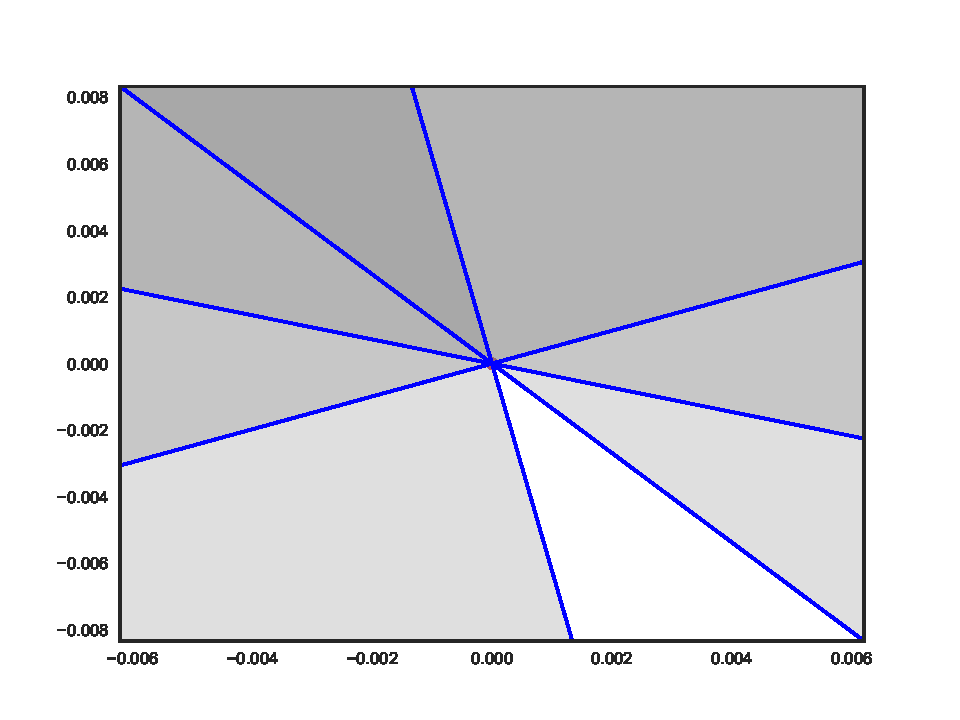
\includegraphics[width=\hsize]{img/toy/relu/conv2d_4-0.pdf}}
    %   \vskip1em
      \subcaptionbox{4th layer}{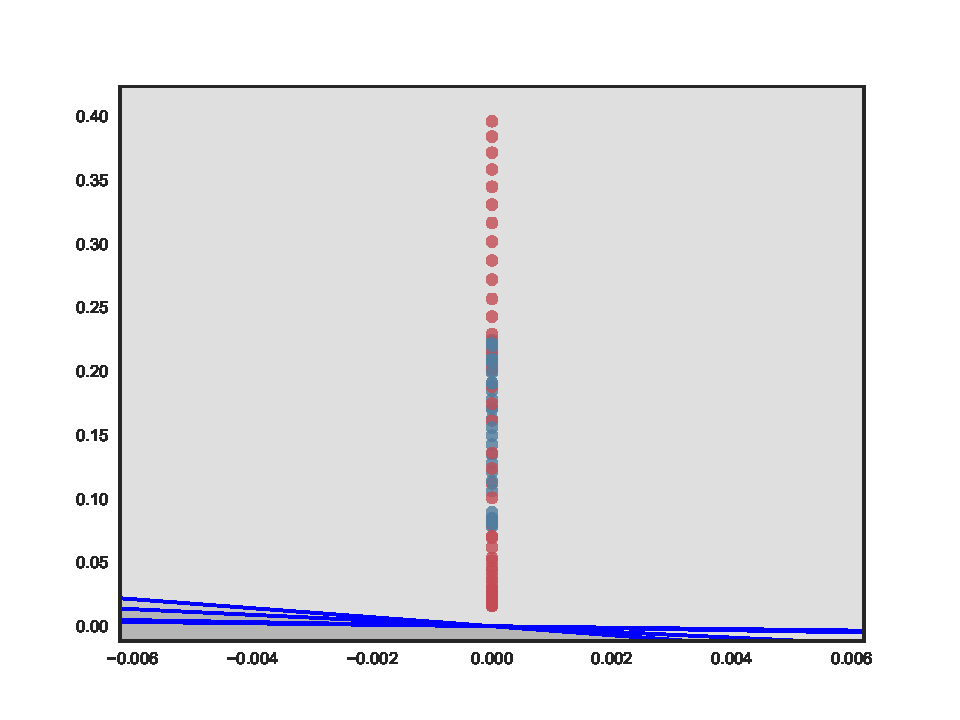
\includegraphics[width=\hsize]{img/toy/relu/conv2d_4-2.pdf}} 
    }
    % \hskip1em
    \parbox{.195\textwidth}{%
      \subcaptionbox{25th layer}{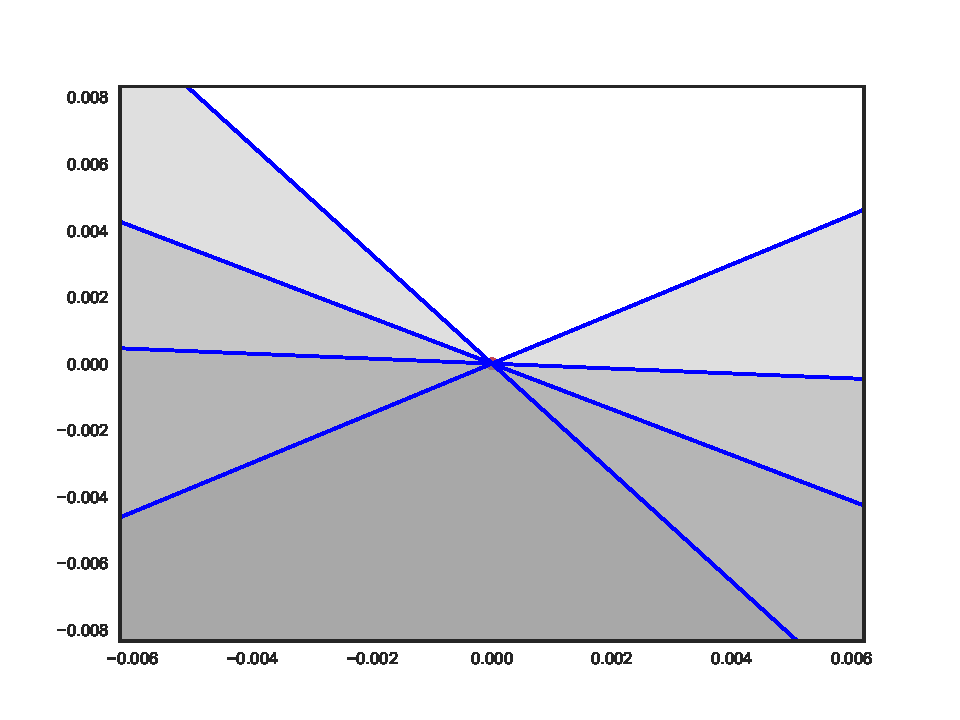
\includegraphics[width=\hsize]{img/toy/relu/conv2d_25-0.pdf}}
    %   \vskip1em
      \subcaptionbox{25th layer}{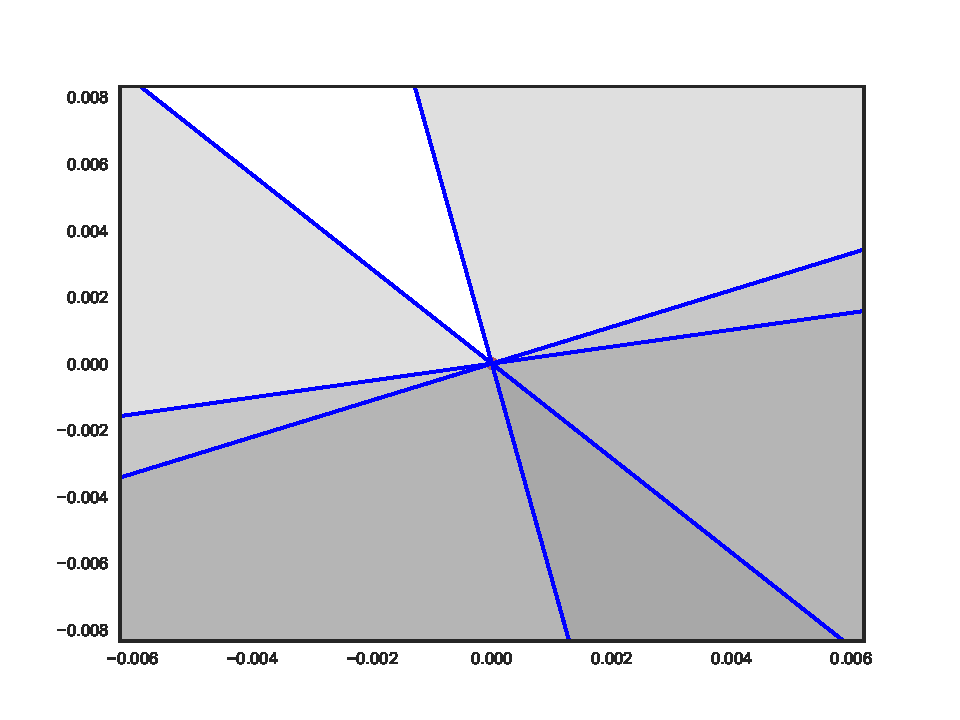
\includegraphics[width=\hsize]{img/toy/relu/conv2d_25-2.pdf}} 
    }
    % \hskip1em
    \parbox{.195\textwidth}{%
      \subcaptionbox{Feature layer}{\includegraphics[width=\hsize]{img/toy/relu/dense_1-0.pdf}}
    %   \vskip1em
      \subcaptionbox{Feature layer}{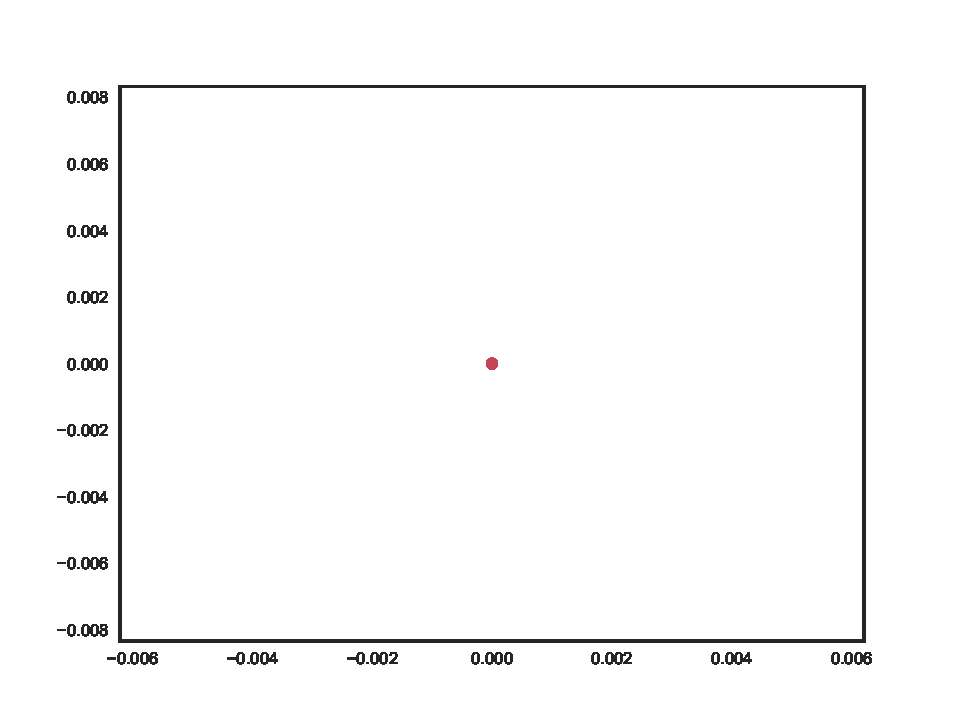
\includegraphics[width=\hsize]{img/toy/relu/dense_1-2.pdf}} 
    }
    % \hskip1em
    \parbox{.195\textwidth}{%
      \subcaptionbox{Output}{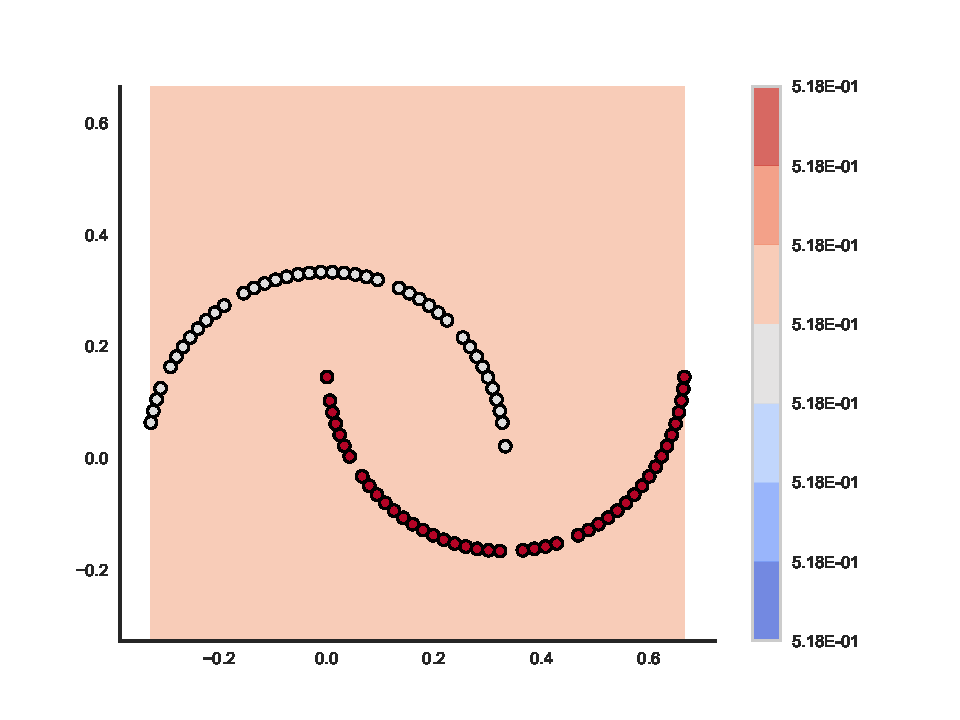
\includegraphics[width=\hsize]{img/toy/relu/output.pdf}}
    }
  }
  \caption{ReLU}
    \label{fig:moonsReLU}
\end{figure*}


Notice how the gradient has changed the separation performed by \ReLU in Figure \ref{fig:moonsReLU} at the input layer (a), but it fails to find a proper representation of use for the upper layers ((b), (c), (d)). The network shrinks the points to zero as they go across the network, to the point where in the 25th layer the entire dataset is in zero. This leads to the total failure to output anything useful (j), which in turn will make impossible to get gradient to overcome the situation. We say that the network is \emph{dead}. We argue that this is because the original placement of the hyperplanes in the layer by the initialization sends to zero a subset of the dataset at a time, so after a number of layers the entire dataset is zero. We undestand that with this all \emph{topological structure} of the network is lost. We relate this phenomena with the lack of smoothness over the transition across layers causing lack of \emph{intuitive} separation but taken to the extreme, described in \cite{hauserAsok}.

\begin{figure*}
  \centering
  \parbox{\textwidth}{
    \parbox{.195\textwidth}{%
      \subcaptionbox{Input layer}{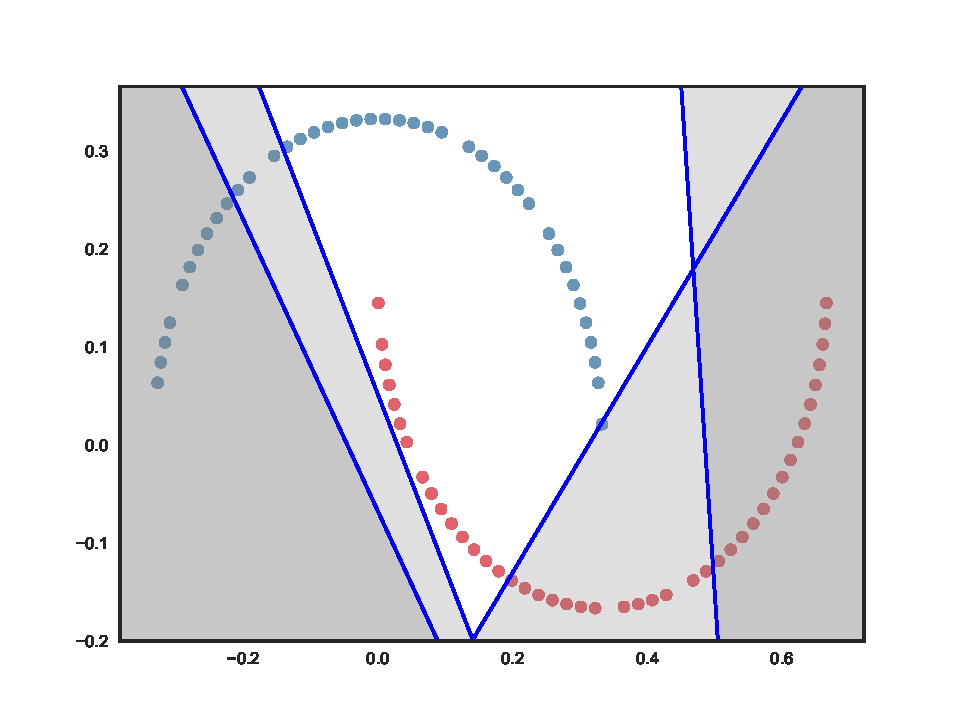
\includegraphics[width=\hsize]{img/toy/relu-bn/conv2d_1-0.pdf}}
    }
    % \hskip1em
    \parbox{.195\textwidth}{%
      \subcaptionbox{4th layer}{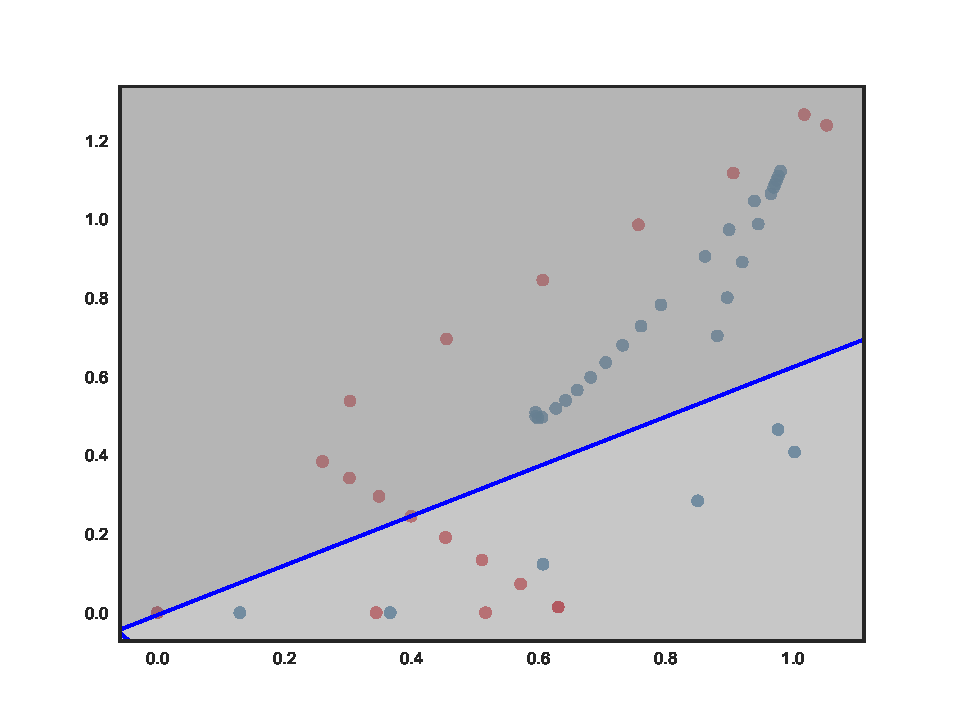
\includegraphics[width=\hsize]{img/toy/relu-bn/conv2d_4-0.pdf}}
    %   \vskip1em
      \subcaptionbox{4th layer}{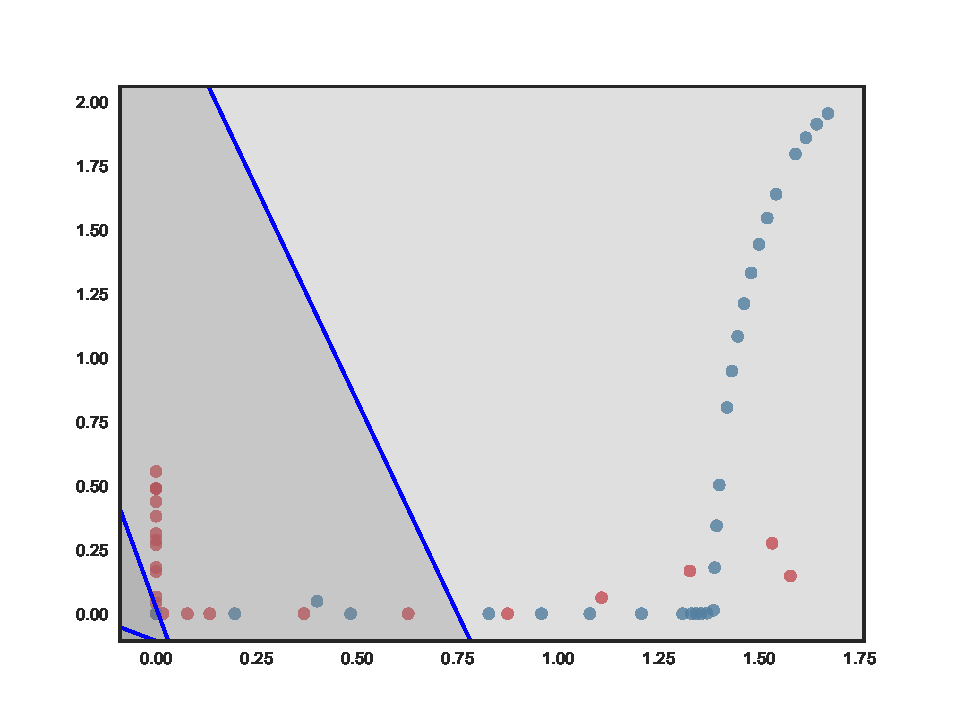
\includegraphics[width=\hsize]{img/toy/relu-bn/conv2d_4-2.pdf}}
    }
    % \hskip1em
    \parbox{.195\textwidth}{%
      \subcaptionbox{25th layer}{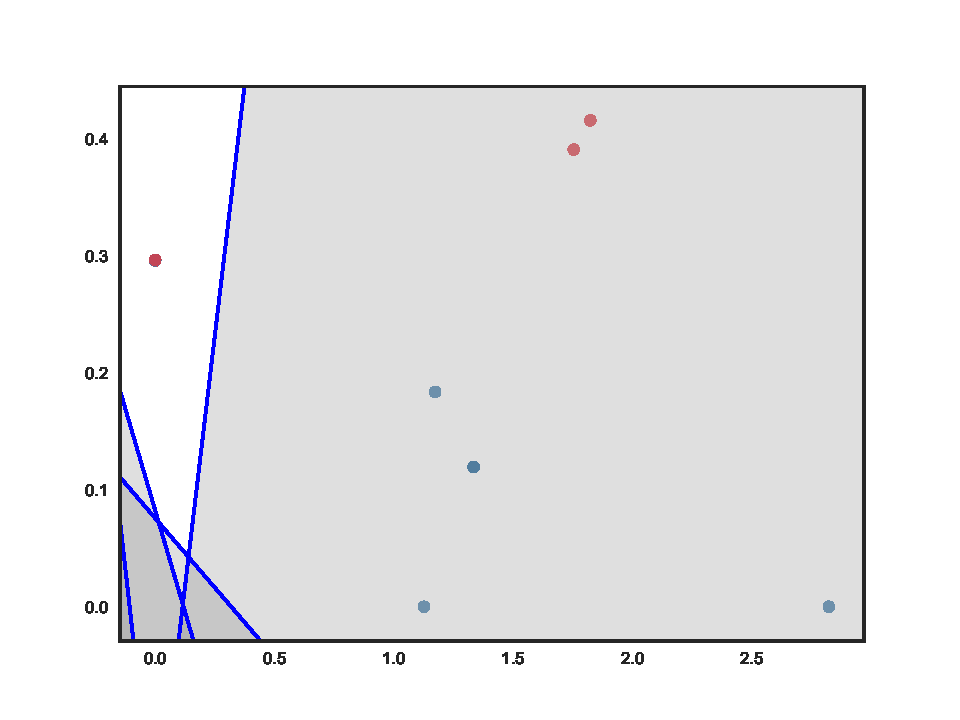
\includegraphics[width=\hsize]{img/toy/relu-bn/conv2d_25-0.pdf}}
    %   \vskip1em
      \subcaptionbox{25th layer}{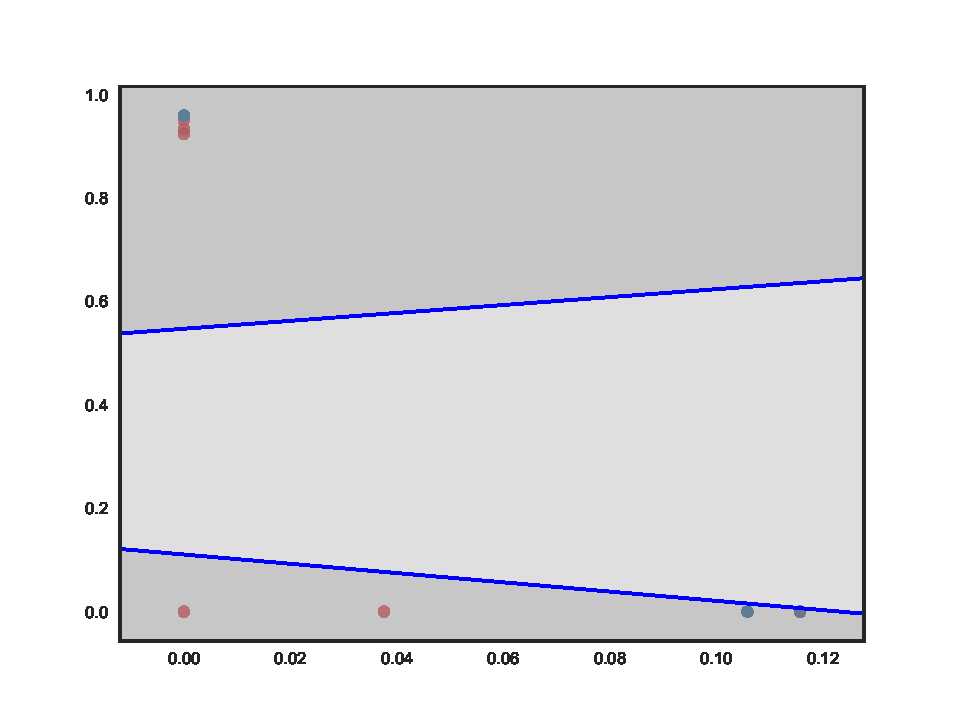
\includegraphics[width=\hsize]{img/toy/relu-bn/conv2d_25-2.pdf}} 
    }
    % \hskip1em
    \parbox{.195\textwidth}{%
      \subcaptionbox{}{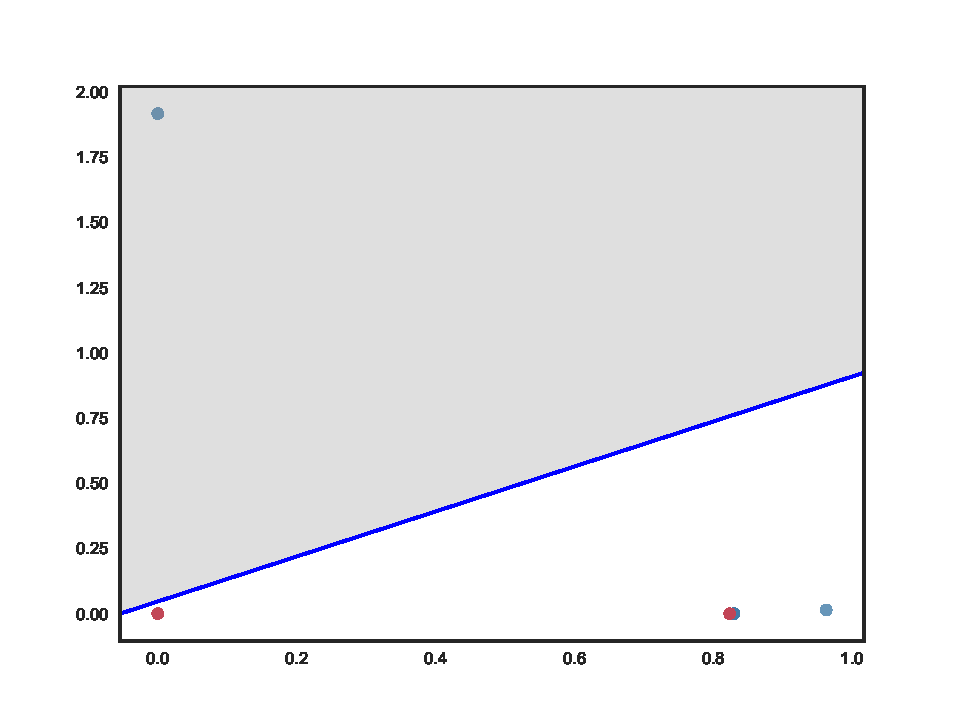
\includegraphics[width=\hsize]{img/toy/relu-bn/dense_1-0.pdf}}
    %   \vskip1em
      \subcaptionbox{}{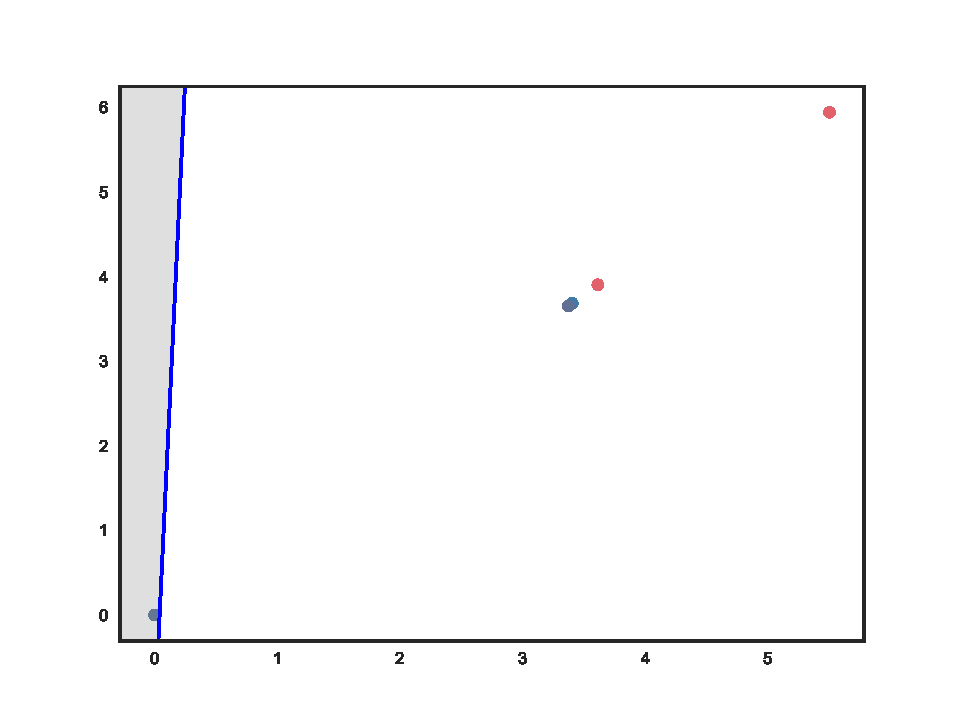
\includegraphics[width=\hsize]{img/toy/relu-bn/dense_1-2.pdf}} 
    }
    % \hskip1em
    \parbox{.195\textwidth}{%
      \subcaptionbox{Output}{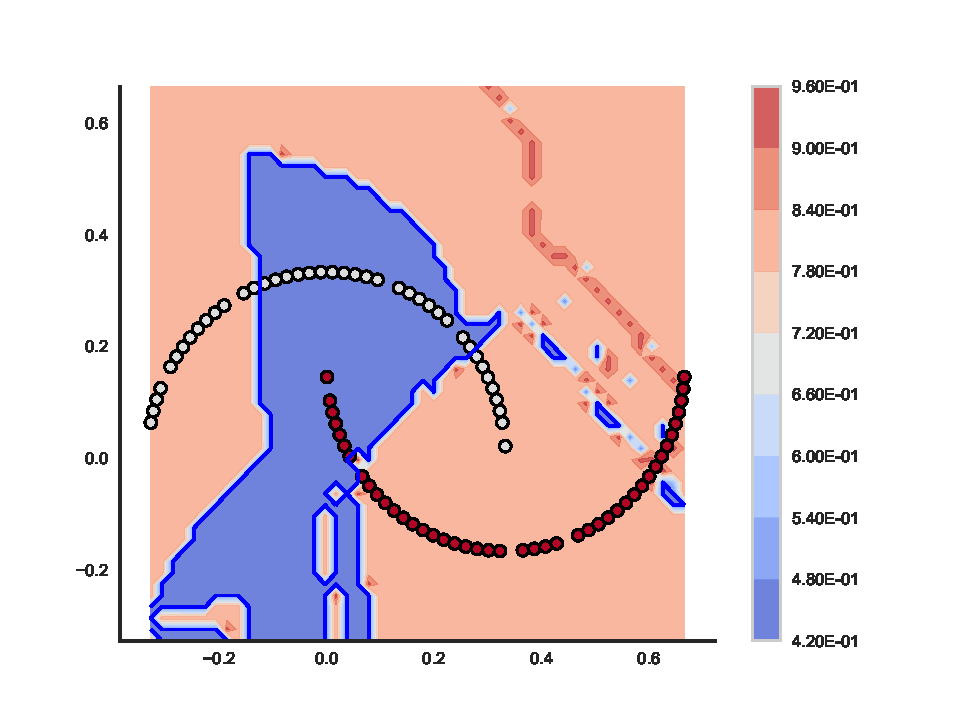
\includegraphics[width=\hsize]{img/toy/relu-bn/output.pdf}}
    }
  }
  \caption{\ReLUBN}
    \label{fig:moonsReLUBN}
\end{figure*}

\ReLUBN fares a bit better since it is able to pull the data out of zero, as we can see in the upper layers ((d), (e), (f), (g)), yet it is still unable to preserve the \emph{topological structure} like \ReLU, which ultimately leads to \emph{topologically mixing} \cite{hirsch2012differential}, in a fashion similar to the \emph{baker's map}. This generates very strange outputs which we can see in (h) whose gradients fail to provide directions to the lower\footnote{We follow an strict platonic view here where abstraction lies above concretion, thus lower layers lie closer to the input and higher layer to the output.} layers to fix the topological structure of the network. 

\begin{figure*}
  \centering
  \parbox{\textwidth}{
    \parbox{.195\textwidth}{%
      \subcaptionbox{Input layer}{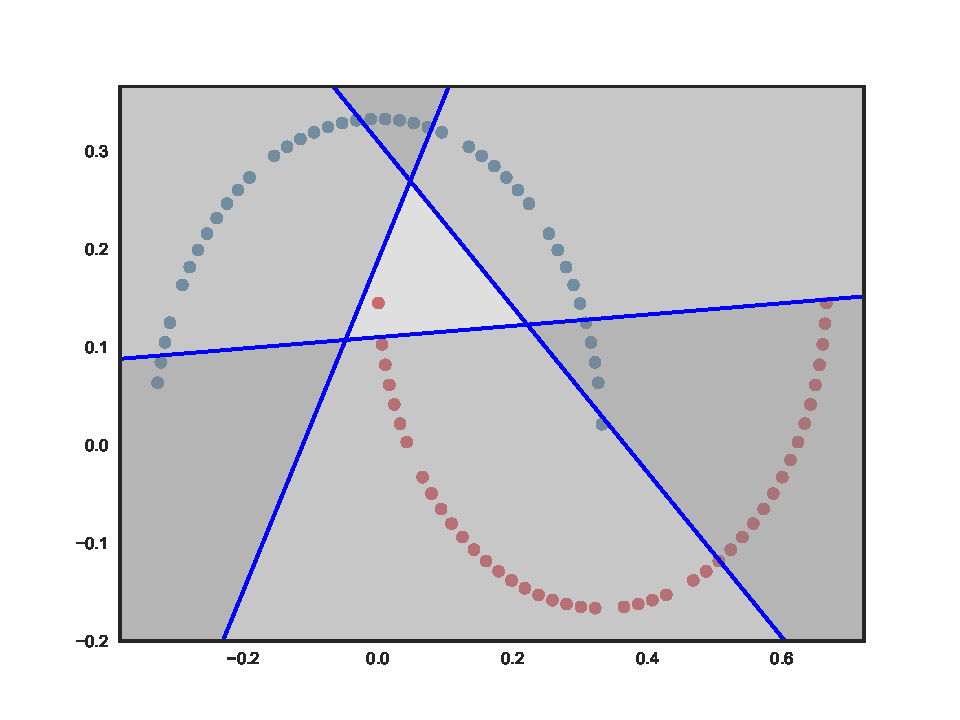
\includegraphics[width=\hsize]{img/toy/layerwise/conv2d_1-0.pdf}}
    }
    % \hskip1em
    \parbox{.195\textwidth}{%
      \subcaptionbox{4th layer}{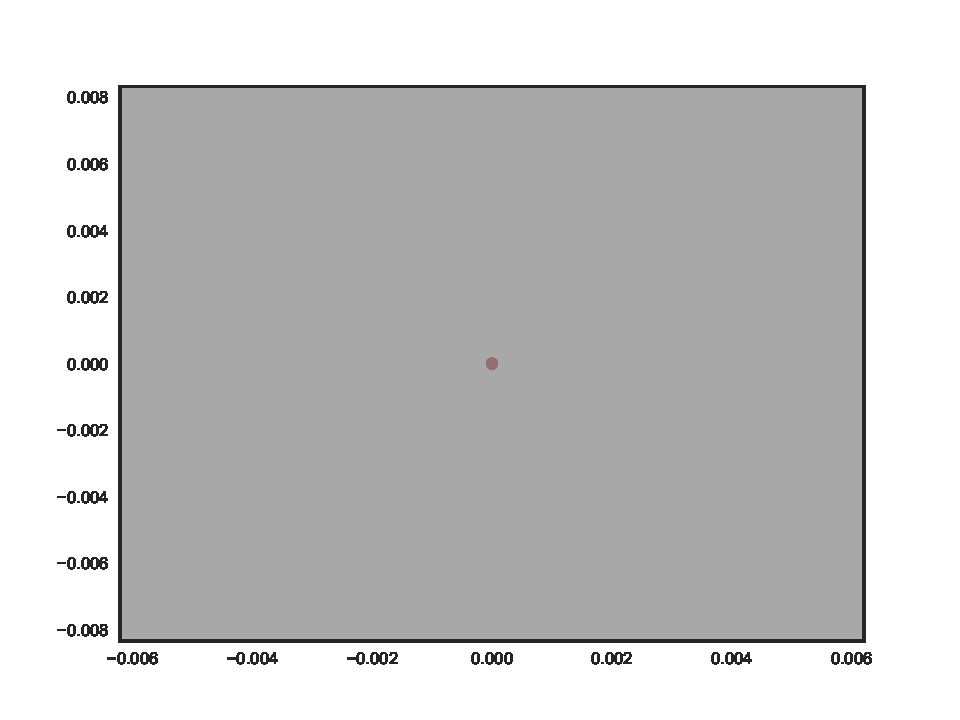
\includegraphics[width=\hsize]{img/toy/layerwise/conv2d_4-0.pdf}}
    %   \vskip1em
      \subcaptionbox{4th layer}{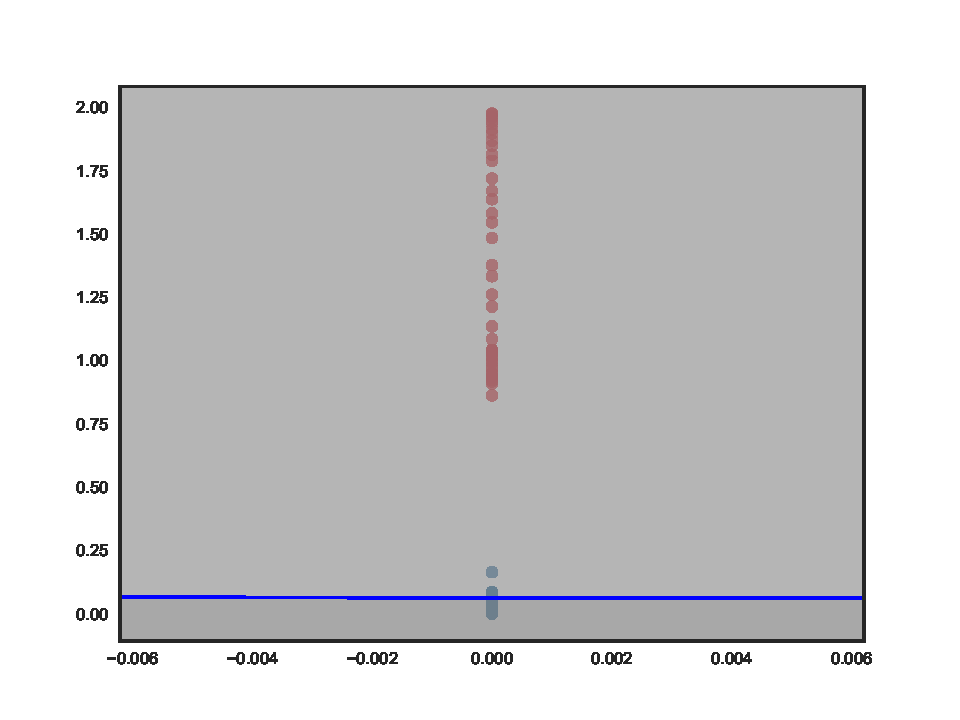
\includegraphics[width=\hsize]{img/toy/layerwise/conv2d_4-2.pdf}} 
    }
    % \hskip1em
    \parbox{.195\textwidth}{%
      \subcaptionbox{25th layer}{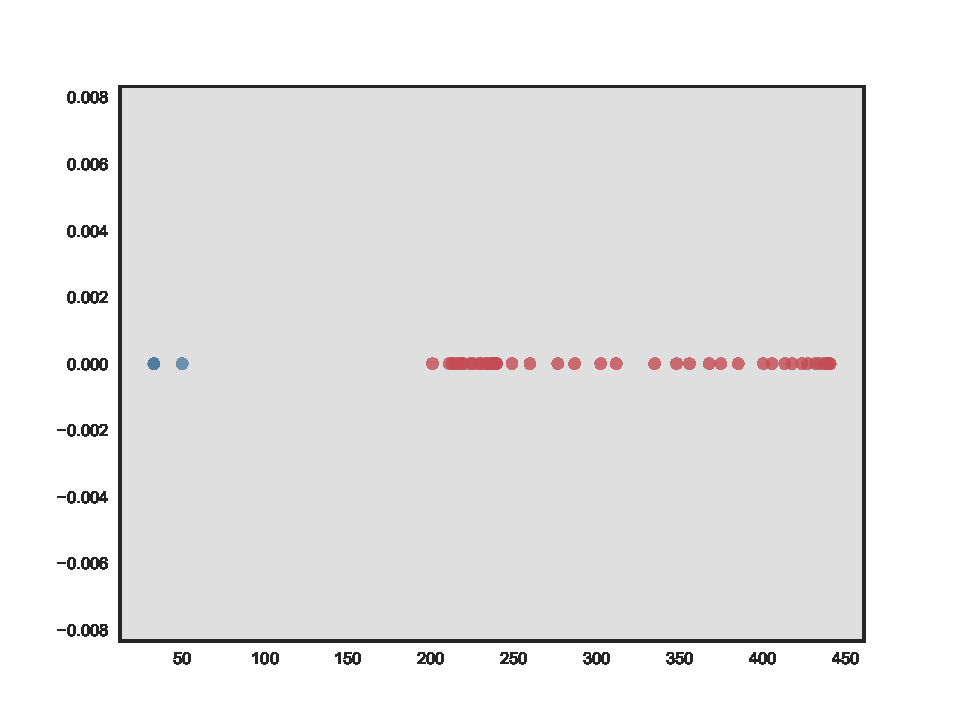
\includegraphics[width=\hsize]{img/toy/layerwise/conv2d_25-0.pdf}}
    %   \vskip1em
      \subcaptionbox{25th layer}{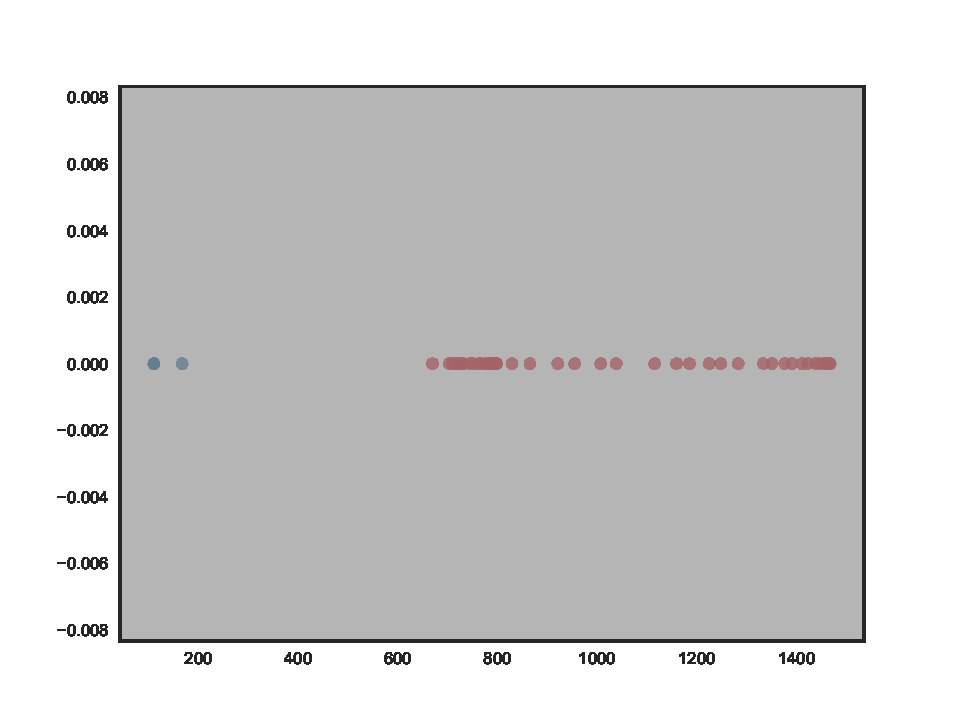
\includegraphics[width=\hsize]{img/toy/layerwise/conv2d_25-2.pdf}} 
    }
    % \hskip1em
    \parbox{.195\textwidth}{%
      \subcaptionbox{Feature layer}{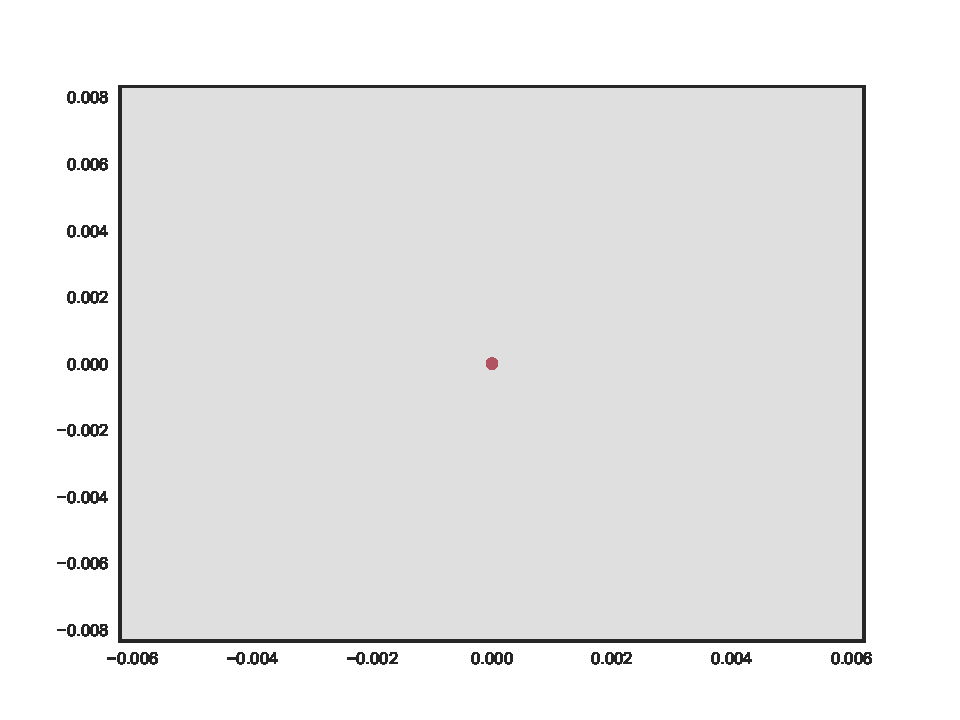
\includegraphics[width=\hsize]{img/toy/layerwise/dense_1-0.pdf}}
    %   \vskip1em
      \subcaptionbox{Feature layer}{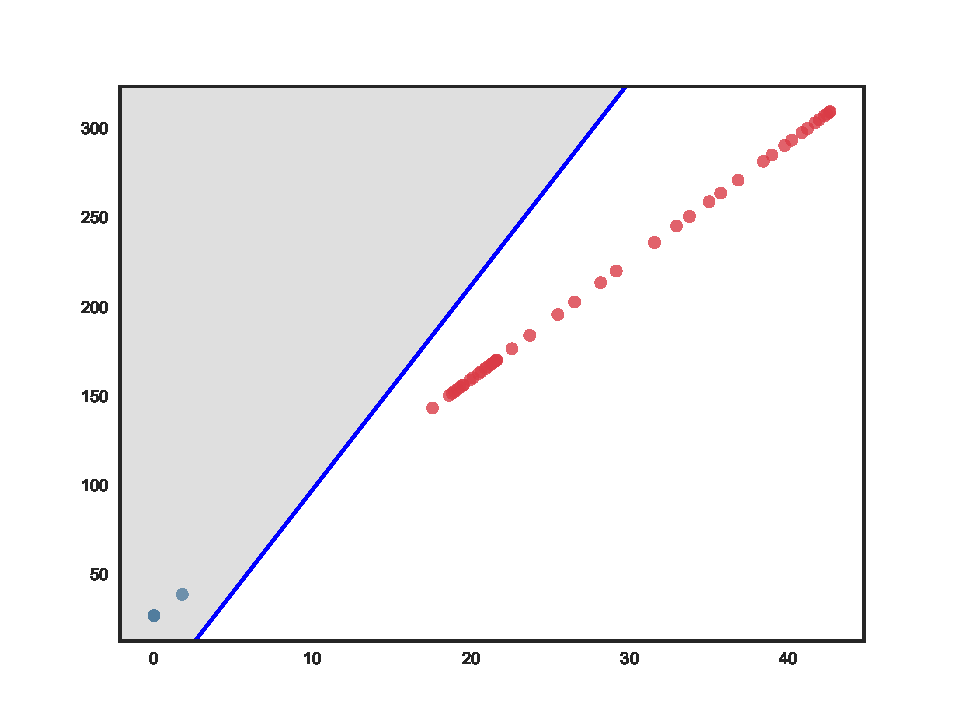
\includegraphics[width=\hsize]{img/toy/layerwise/dense_1-2.pdf}} 
    }
    % \hskip1em
    \parbox{.195\textwidth}{%
      \subcaptionbox{Output}{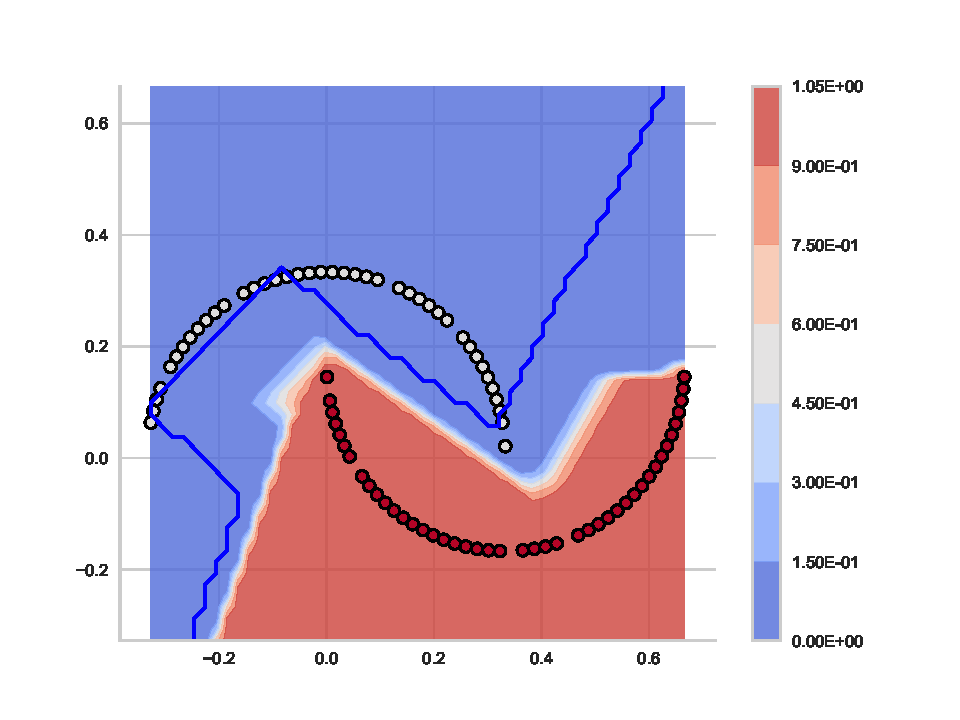
\includegraphics[width=\hsize]{img/toy/layerwise/output.pdf}}
    }
  }
    \caption{\SepLayer}
    \label{fig:moonsLayerwise}
\end{figure*}


In the other hand, our relaxed version of our proposal \SepLayer, see Figure \ref{fig:moonsLayerwise}, is able to solve the problem (h). We find how is able to propagate the information needed for the lower layers to perform the separation, so we can see at (k) how the separating planes are much better placed, so by the bottom layers (c) the problem is already solved and the rest of layers simply forward upwards ((d), (e)). Since our formulation \SepLayer is a relaxed version of \SepUnit we allow are redundant and dead units. Notice how the entire space is colored in different shades of gray, showing how at (d) least one unit is effectively operating in linear mode, thus proving how in certain situations affine units might be useful by forwarding information into deeper layers. 

\begin{figure*}
  \centering
     % Unitwise
  \parbox{\textwidth}{
    \parbox{.195\textwidth}{%
      \subcaptionbox{Input layer}{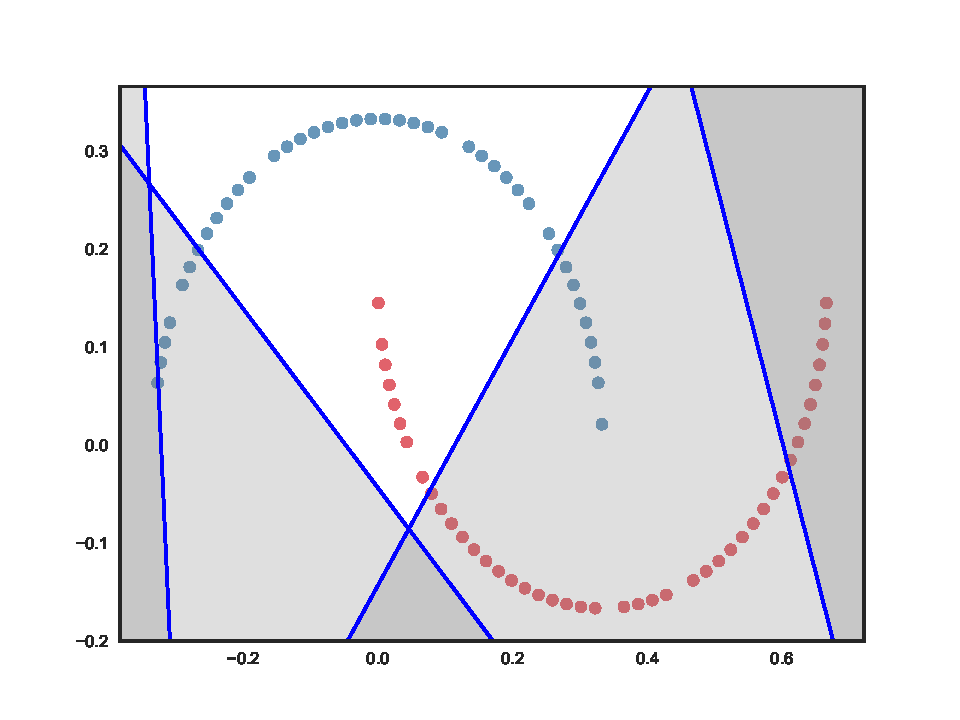
\includegraphics[width=\hsize]{img/toy/unitwise/conv2d_1-0.pdf}}
    }
    % \hskip1em
    \parbox{.195\textwidth}{%
      \subcaptionbox{4th layer}{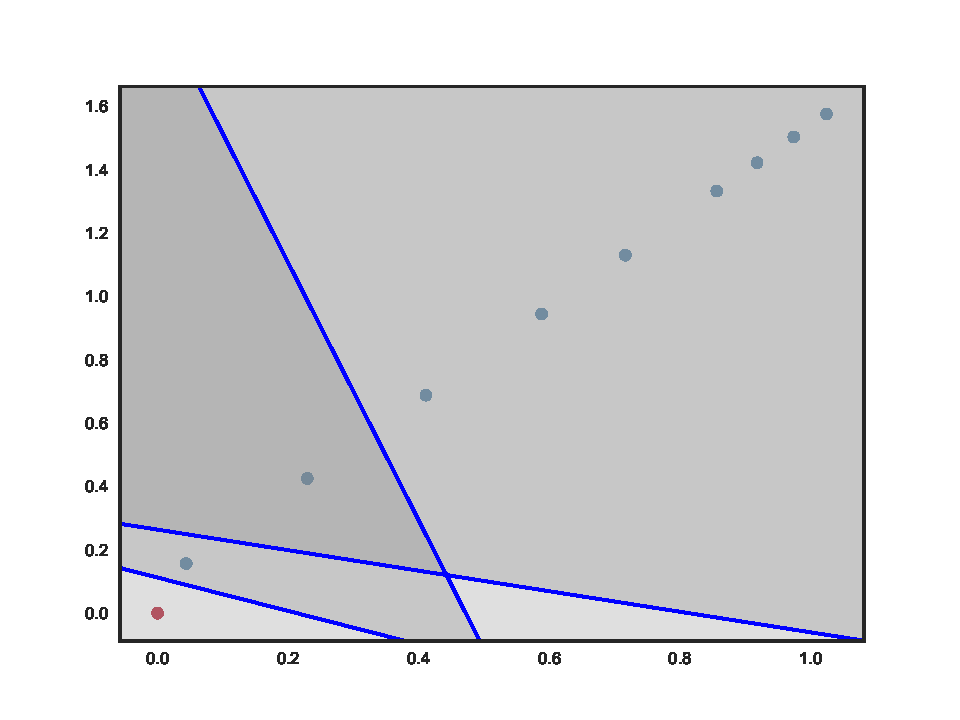
\includegraphics[width=\hsize]{img/toy/unitwise/conv2d_4-0.pdf}}
    %   \vskip1em
      \subcaptionbox{4th layer}{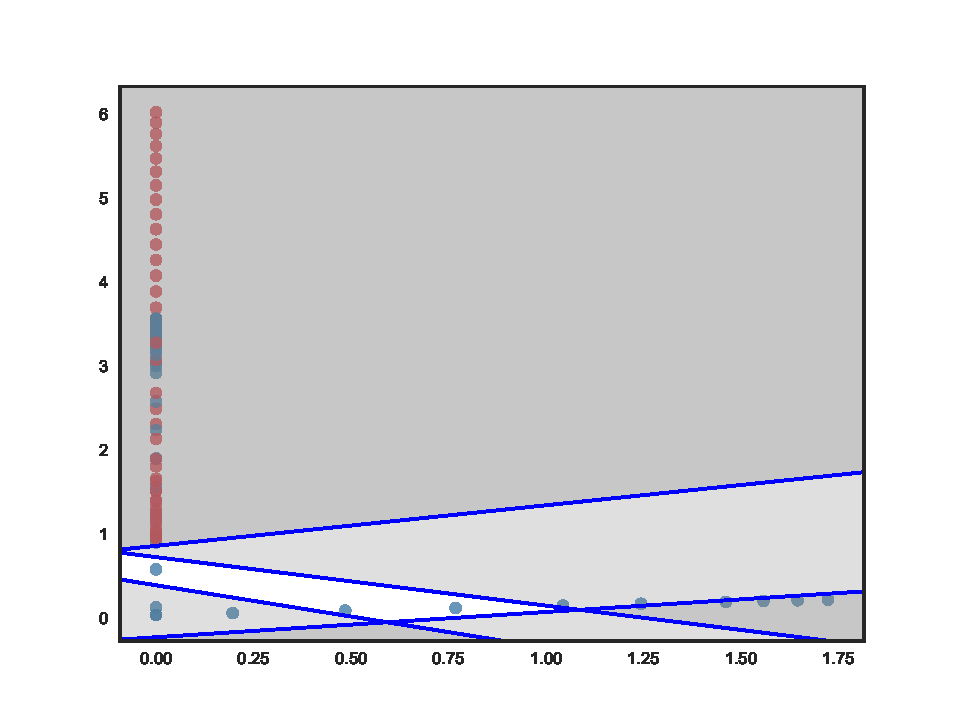
\includegraphics[width=\hsize]{img/toy/unitwise/conv2d_4-2.pdf}} 
    }
    % \hskip1em
    \parbox{.195\textwidth}{%
      \subcaptionbox{25th layer}{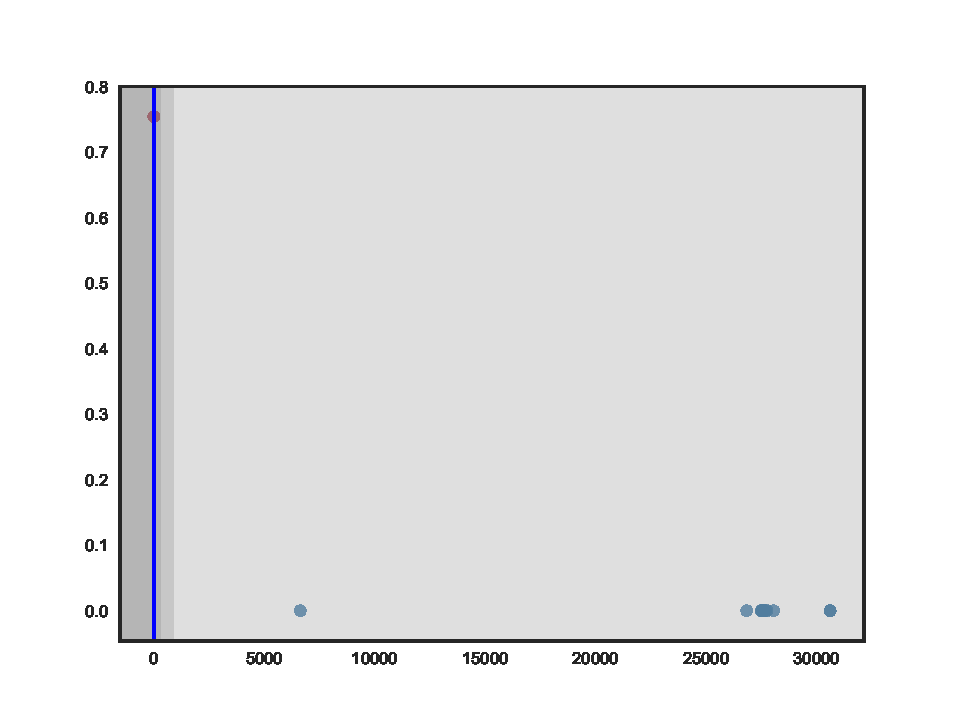
\includegraphics[width=\hsize]{img/toy/unitwise/conv2d_25-0.pdf}}
    %   \vskip1em
      \subcaptionbox{25th layer}{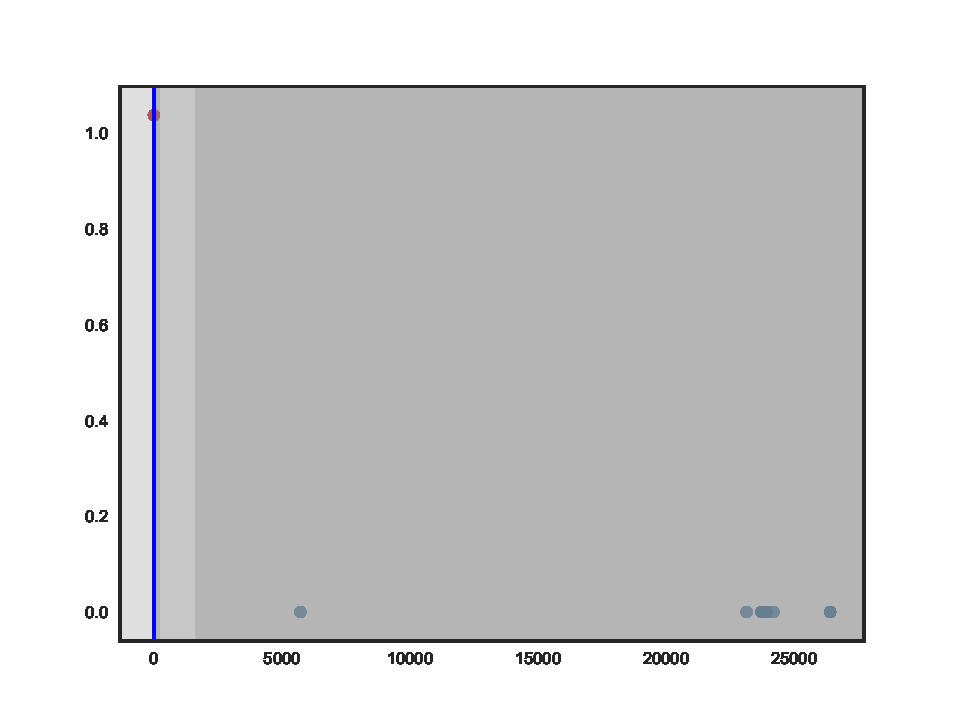
\includegraphics[width=\hsize]{img/toy/unitwise/conv2d_25-2.pdf}} 
    }
    % \hskip1em
    \parbox{.195\textwidth}{%
      \subcaptionbox{Feature layer}{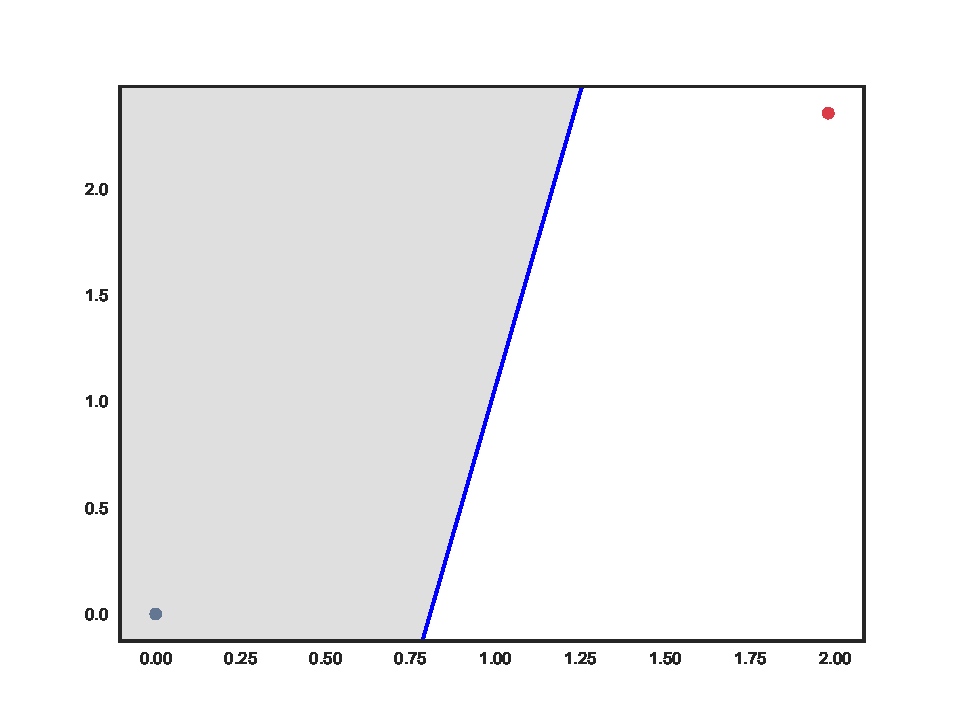
\includegraphics[width=\hsize]{img/toy/unitwise/dense_1-0.pdf}}
    %   \vskip1em
      \subcaptionbox{Feature layer}{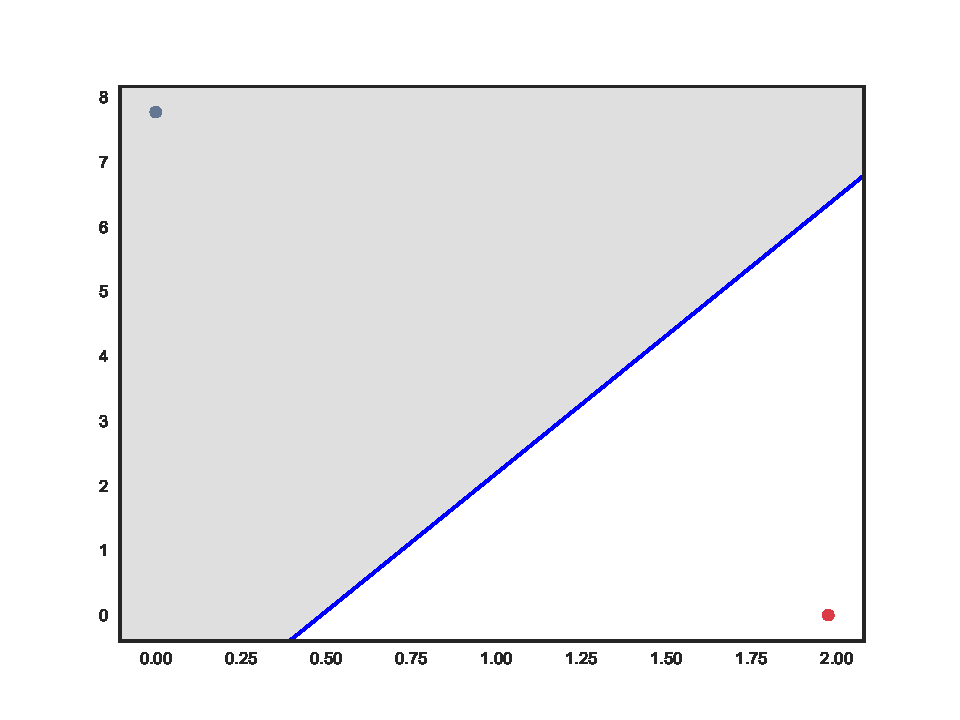
\includegraphics[width=\hsize]{img/toy/unitwise/dense_1-2.pdf}} 
    }
    % \hskip1em
    \parbox{.195\textwidth}{%
      \subcaptionbox{Output}{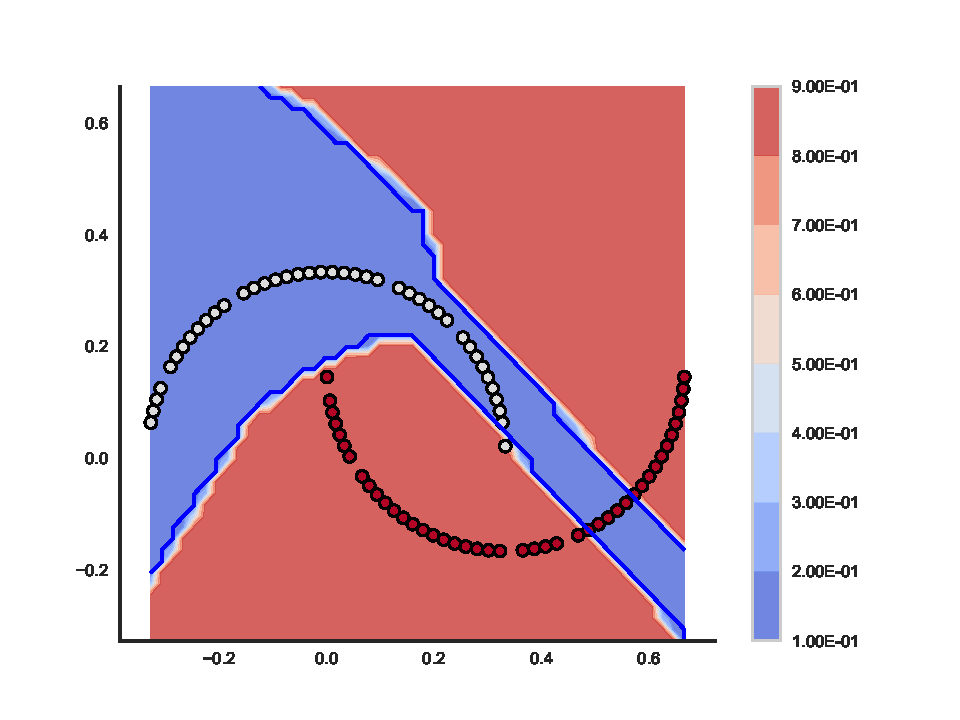
\includegraphics[width=\hsize]{img/toy/unitwise/output.pdf}}
    }
  }
  \caption{\SepUnit}
    \label{fig:moonsUnitwise}
\end{figure*}


Figure \ref{fig:moonsUnitwise} presents the results of \SepUnit. We find that the solution achieved is suboptimal, for which we blame on the excessive non-linearity induced by the constraint, preventing to forward solutions found in the lower layers to the output or allowing points with no activation, as we explained in \ref{eq:unitFail}. However, the boundary found is still quite \emph{intuitive}, in terms of \cite{hauserAsok}. Notice how the feature layer \ref{fig:moonsUnitwise}(f,g) is much more polarized than \SepLayer \ref{fig:moonsLayerwise}(f,g), and similar to \ReLUBN \ref{fig:moonsReLUBN}(f,g), although the representation at layer 25 (d,e) is richer and the output is much better.

\begin{figure*}
  \centering
  %Pointwise
  \parbox{\textwidth}{
    \parbox{.195\textwidth}{%
      \subcaptionbox{Input layer}{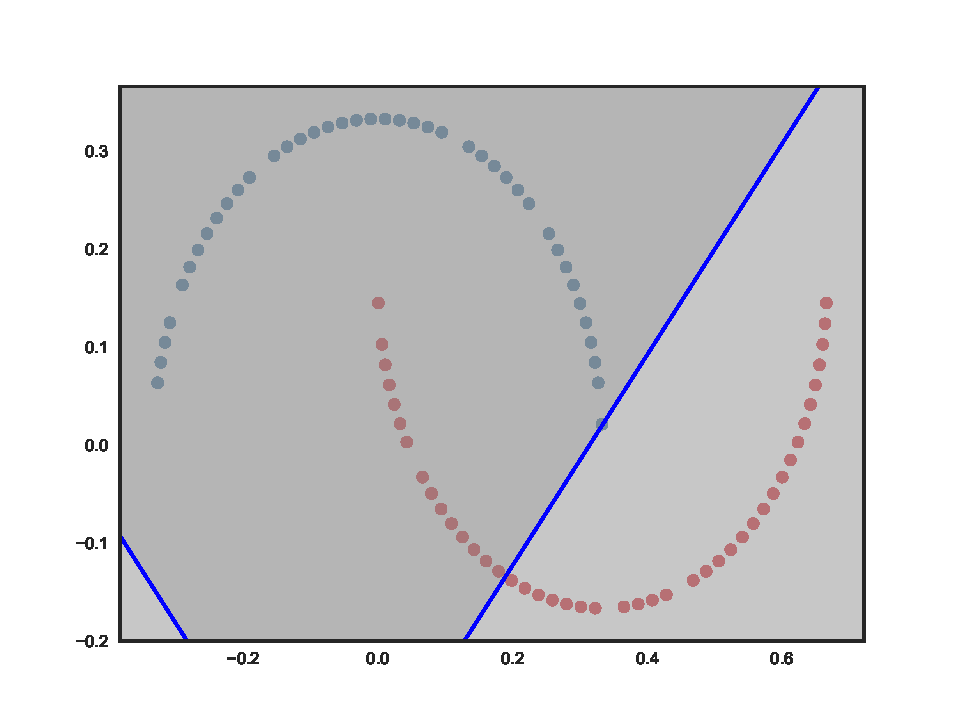
\includegraphics[width=\hsize]{img/toy/pointwise/conv2d_1-0.pdf}}
    }
    % \hskip1em
    \parbox{.195\textwidth}{%
      \subcaptionbox{4th layer}{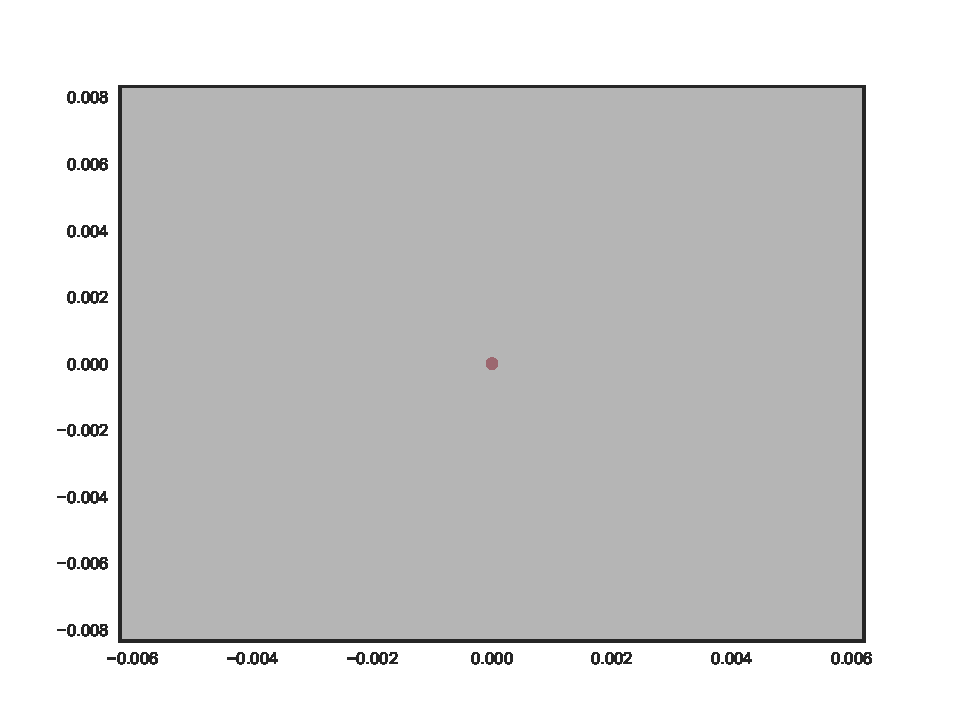
\includegraphics[width=\hsize]{img/toy/pointwise/conv2d_4-0.pdf}}
    %   \vskip1em
      \subcaptionbox{4th layer}{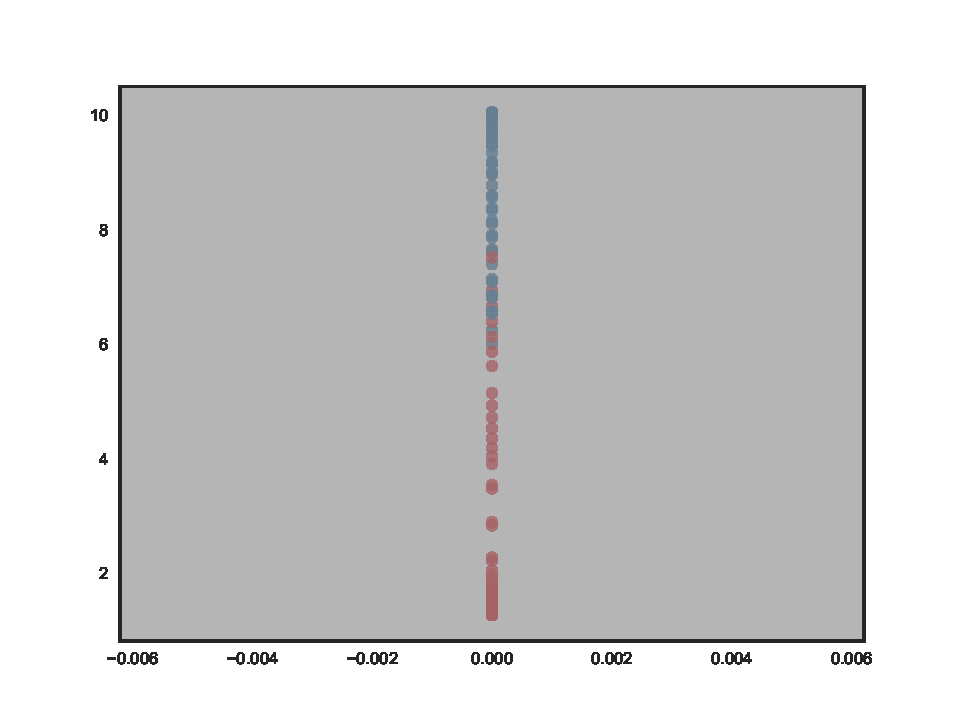
\includegraphics[width=\hsize]{img/toy/pointwise/conv2d_4-2.pdf}} 
    }
    % \hskip1em
    \parbox{.195\textwidth}{%
      \subcaptionbox{25th layer}{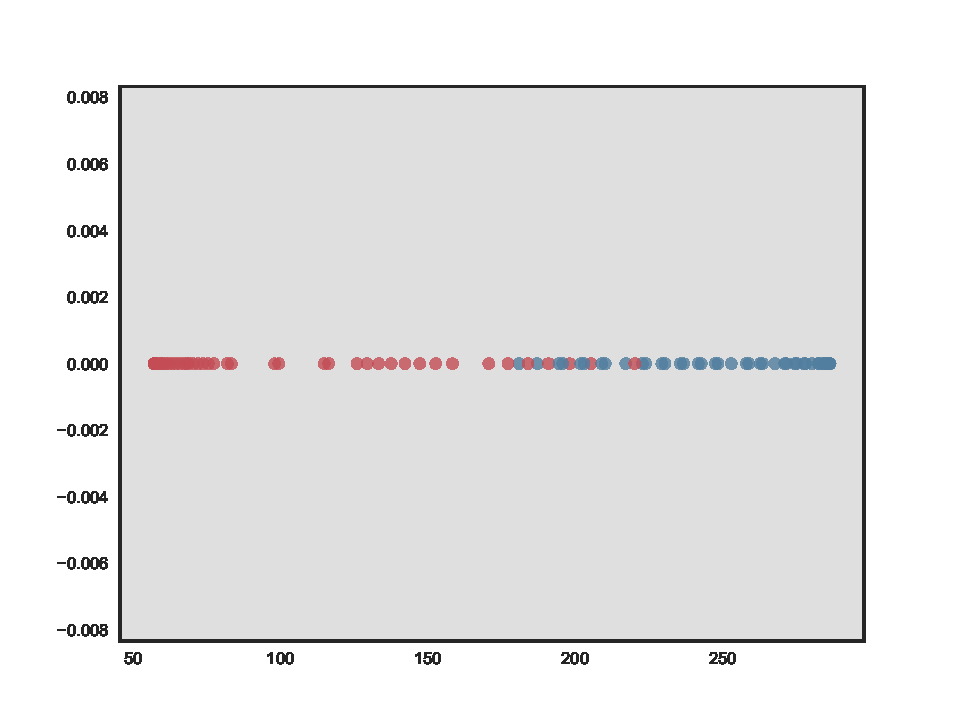
\includegraphics[width=\hsize]{img/toy/pointwise/conv2d_25-0.pdf}}
    %   \vskip1em
      \subcaptionbox{25th layer}{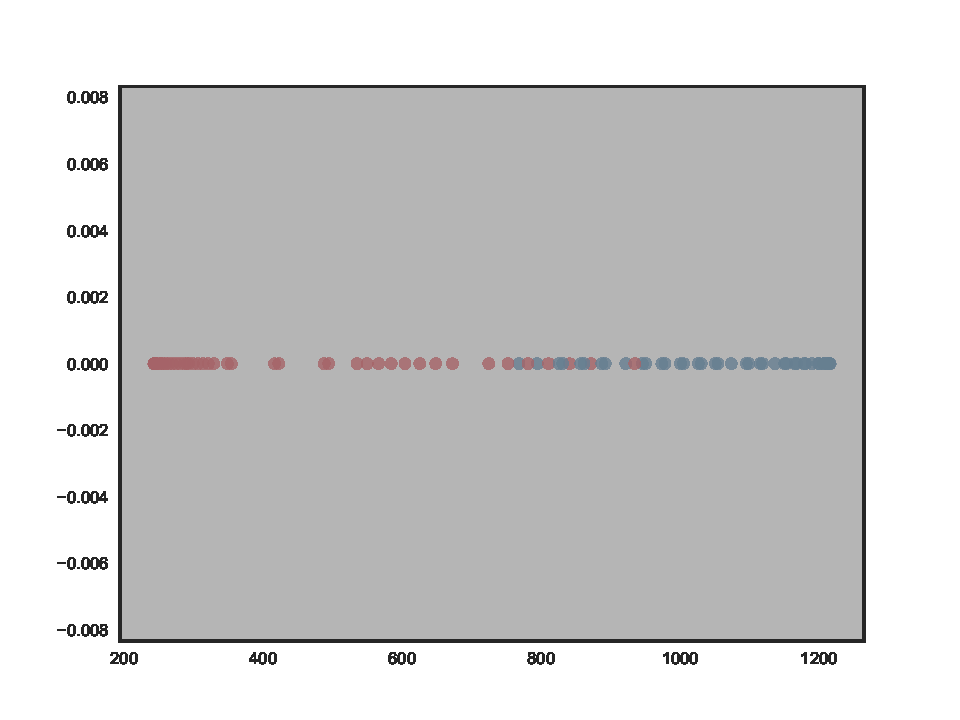
\includegraphics[width=\hsize]{img/toy/pointwise/conv2d_25-2.pdf}} 
    }
    % \hskip1em
    \parbox{.195\textwidth}{%
      \subcaptionbox{}{\includegraphics[width=\hsize]{img/toy/pointwise/dense_1-0.pdf}}
    %   \vskip1em
      \subcaptionbox{}{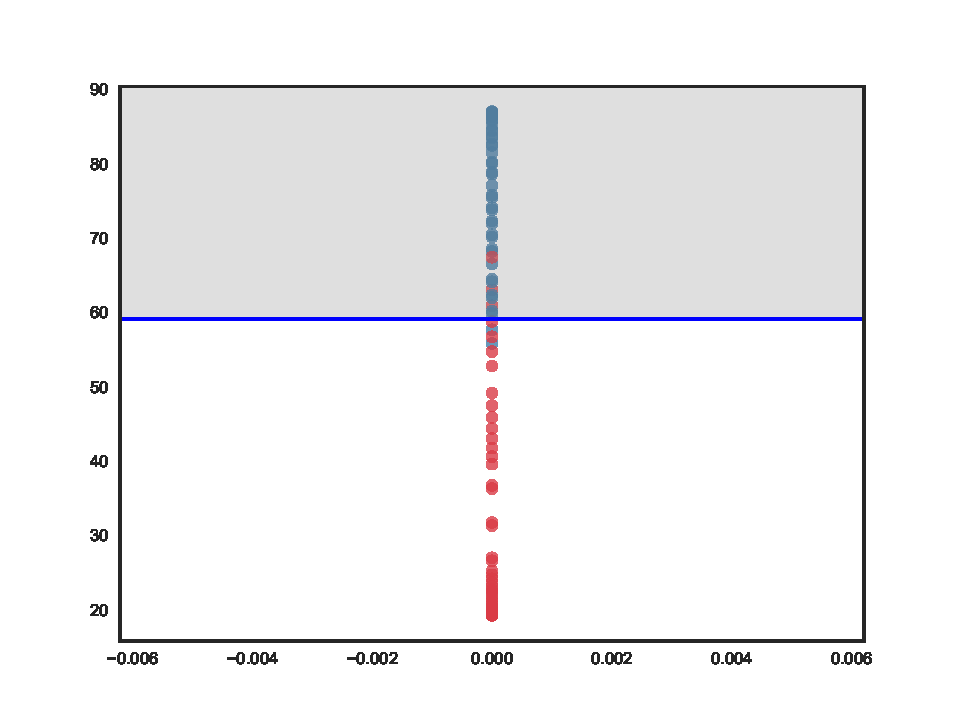
\includegraphics[width=\hsize]{img/toy/pointwise/dense_1-2.pdf}} 
    }
    % \hskip1em
    \parbox{.195\textwidth}{%
      \subcaptionbox{Output}{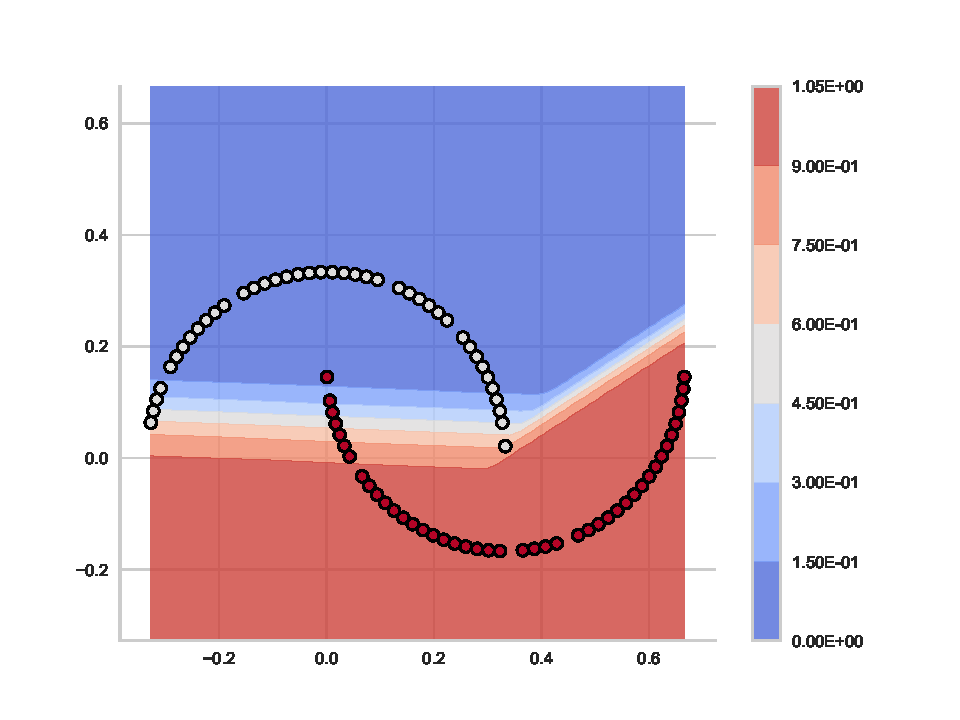
\includegraphics[width=\hsize]{img/toy/pointwise/output.pdf}}
    }
  }
  \caption{\SepPoint}
    \label{fig:moonsPointwise}
\end{figure*}

The constraint \SepPoint is shown at Figure \ref{fig:moonsPointwise}. We see how it effectively propagates the data \emph{topological structure} up to the output of the network ((e), (d), (f), (g)), but as the only requirement that for each point at least one unit is activated and another not this can be fulfilled with an affine unit, so the solution remains almost linear (h). 

\begin{figure*}
  \centering
   \parbox{\textwidth}{
    \parbox{.195\textwidth}{%
      \subcaptionbox{Input layer}{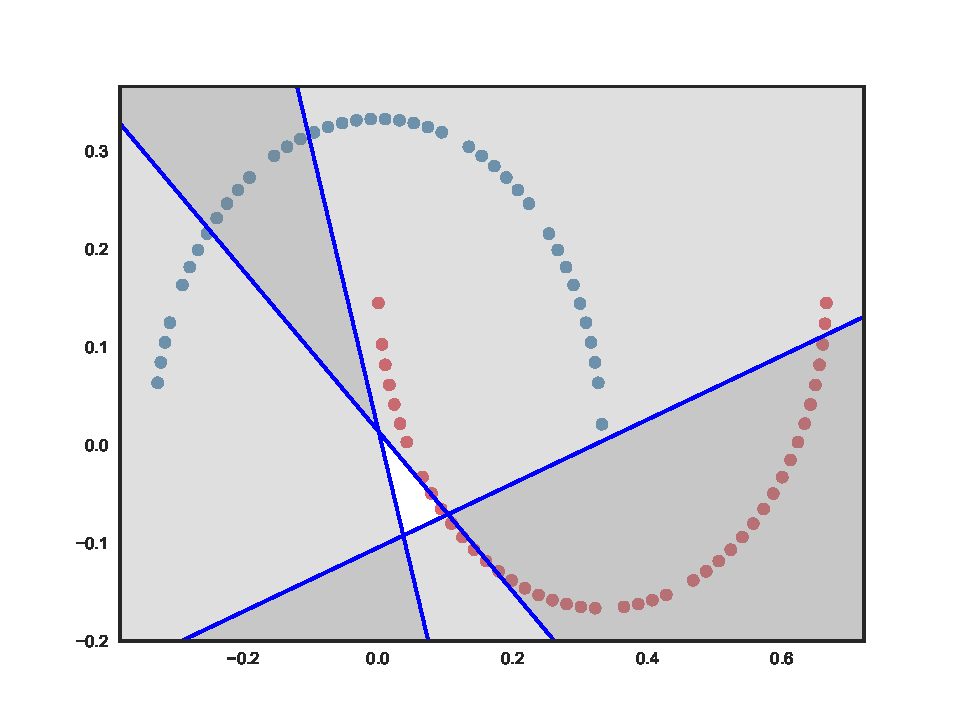
\includegraphics[width=\hsize]{img/toy/unitpointwise/conv2d_1-0.pdf}}
    }
    % \hskip1em
    \parbox{.195\textwidth}{%
      \subcaptionbox{4th layer}{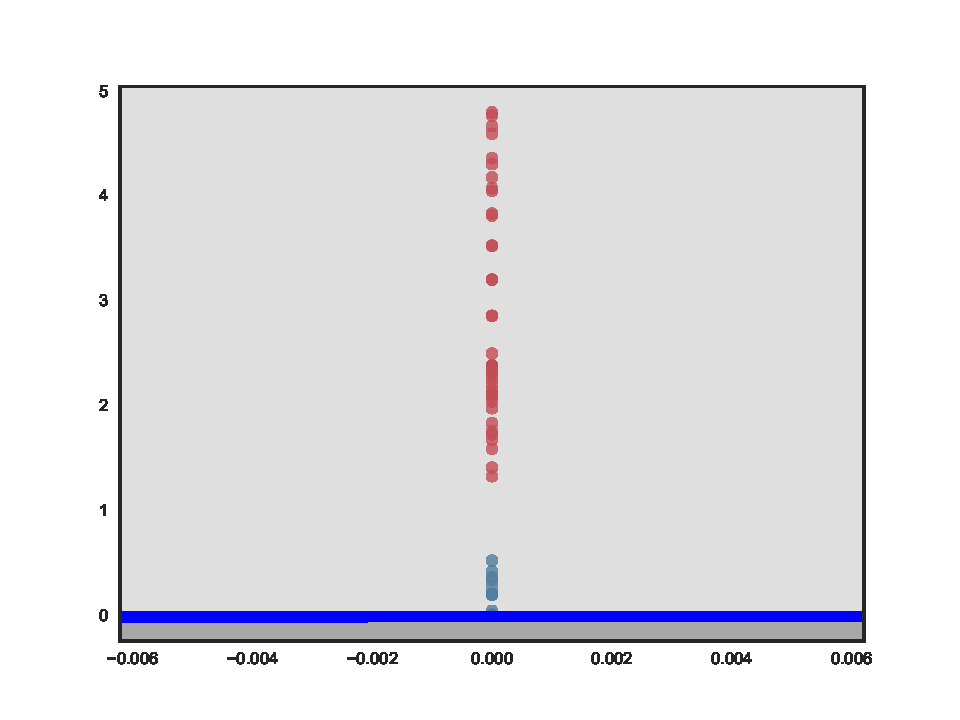
\includegraphics[width=\hsize]{img/toy/unitpointwise/conv2d_4-0.pdf}}
    %   \vskip1em
      \subcaptionbox{4th layer}{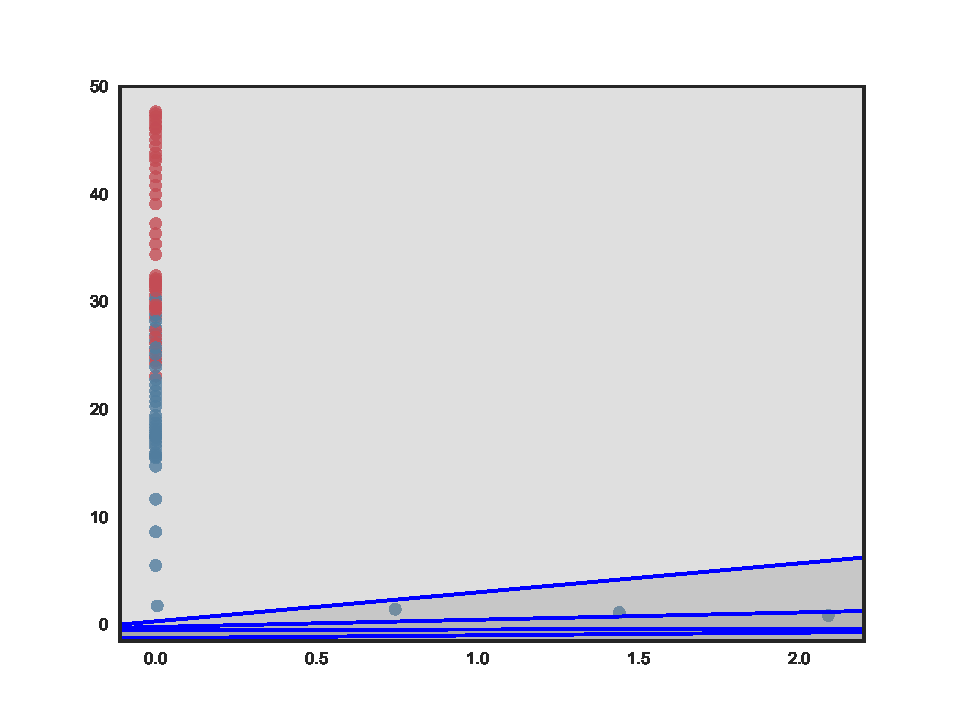
\includegraphics[width=\hsize]{img/toy/unitpointwise/conv2d_4-2.pdf}} 
    }
    % \hskip1em
    \parbox{.195\textwidth}{%
      \subcaptionbox{25th layer}{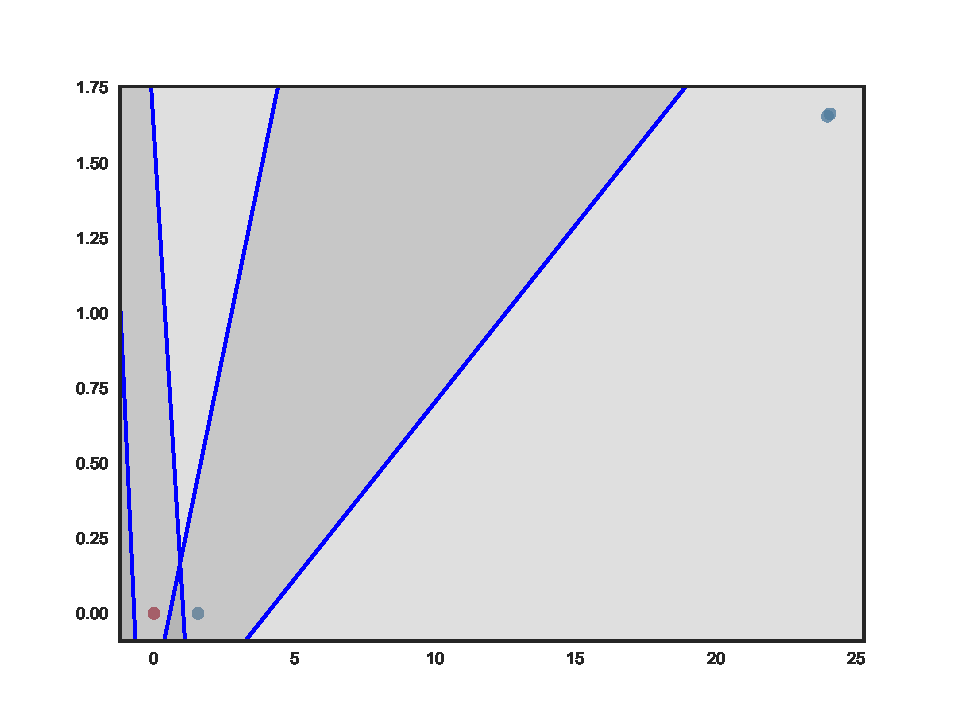
\includegraphics[width=\hsize]{img/toy/unitpointwise/conv2d_25-0.pdf}}
    %   \vskip1em
      \subcaptionbox{25th layer}{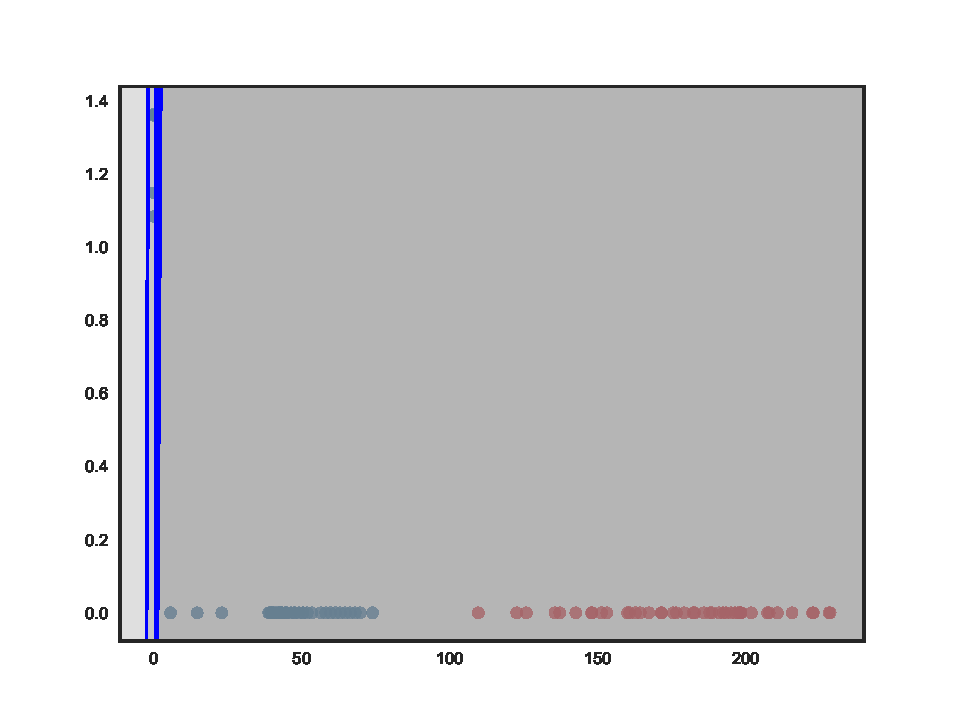
\includegraphics[width=\hsize]{img/toy/unitpointwise/conv2d_25-2.pdf}} 
    }
    % \hskip1em
    \parbox{.195\textwidth}{%
      \subcaptionbox{Feature layer}{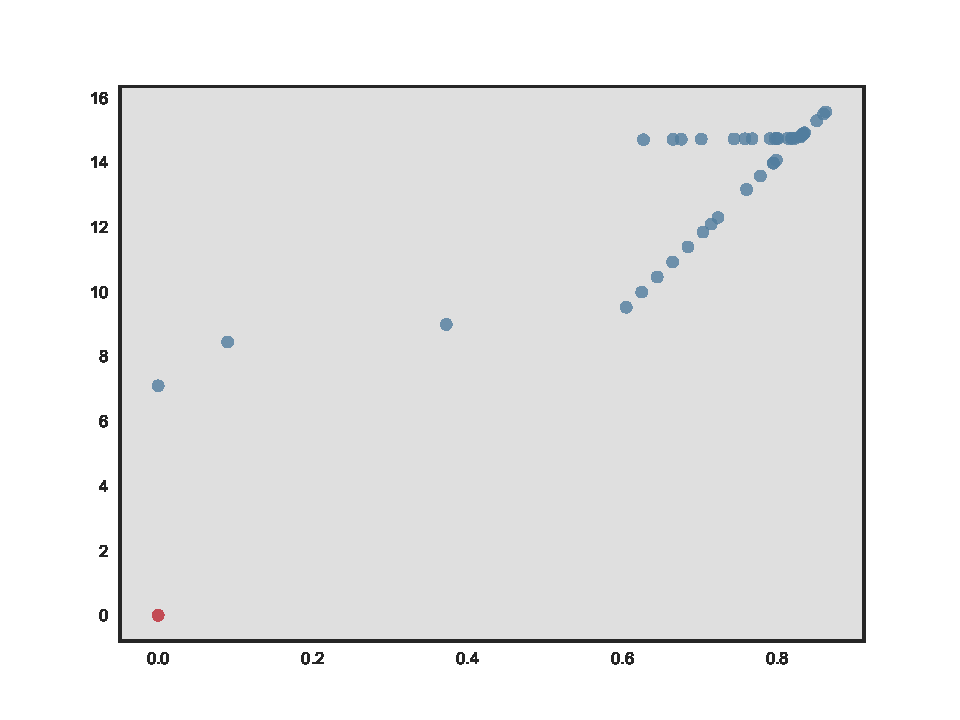
\includegraphics[width=\hsize]{img/toy/unitpointwise/dense_1-0.pdf}}
    %   \vskip1em
      \subcaptionbox{Feature layer}{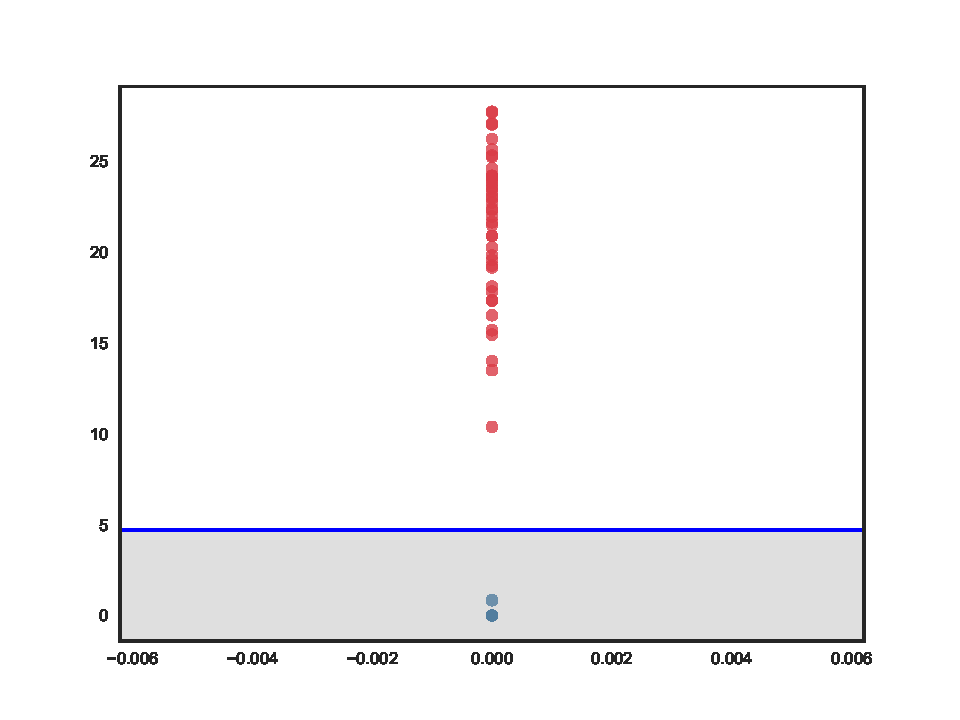
\includegraphics[width=\hsize]{img/toy/unitpointwise/dense_1-2.pdf}} 
    }
    % \hskip1em
    \parbox{.195\textwidth}{%
      \subcaptionbox{Output}{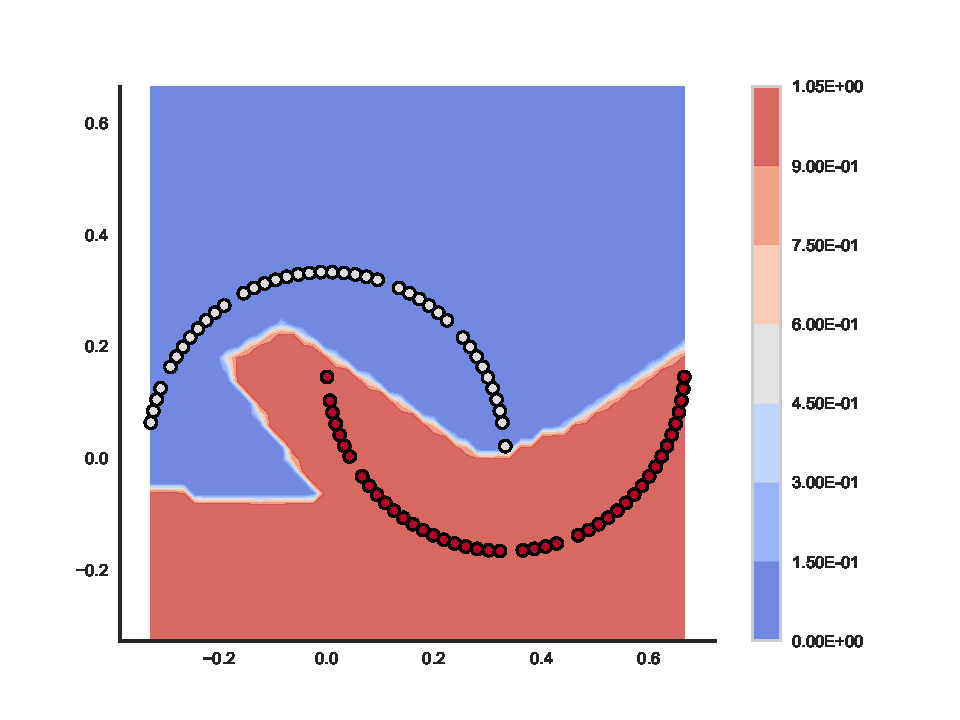
\includegraphics[width=\hsize]{img/toy/unitpointwise/output.pdf}}
    }
  }

    \caption{\SepUnitPoint}
    \label{fig:moonsUnitpointwise}
\end{figure*}

Finally, combining \SepUnit with \SepPoint in \SepUnitPoint effectively separates the classes at Figure \ref{fig:moonsUnitpointwise} (h). The solution found is a bit different from \SepLayer at Figure \ref{fig:moonsLayerwise}(h). We argue that this is due the increased non-linearity of \SepUnit over \SepLayer.

\subsection{The Effect of Constraint Loss}\label{subsec:effectConstraintLoss}

One interesting matter is to understand which effect has the separation constraint by itself, without loss functional. Therefore, we train the same network and hyperparameters than the previous experiment  \ref{subsec:classification}. Then we optimize only the constraints without any other loss. We use \ReLU and \ReLUBN for comparison purposes. 

We find that both \ReLU and \ReLUBN tend concentrate all the data whereas \SepUnitPoint and \SepLayer are able to preserve topological structure, see figure \ref{fig:init}. This explains the failure in \ref{fig:moonsReLU} and \ref{fig:moonsReLUBN}. 
In the other hand, we find how \SepLayer connects the output with in the input by sort of linearizing the network in figures \ref{fig:layerwiseInit501} and \ref{fig:layerwiseInit501}, thus outputting something very similar to a linear classifier. This is consistent with \cite{batchnormGradientExplosion}, where the authors claim that the network performs best as the units work closest to the linear regime. 
\SepUnitPoint output in figures \ref{fig:unitpointInit501} and \ref{fig:unitpointInit502} is less smooth than \SepLayer but still reasonable showing connectivity among the points, proof that topological structure is preserved up to some extent. Notice how the shape of the input layer is quite similar to the final solution found in Figure \ref{fig:moonsUnitpointwise}(a) when using a loss functional, but the feature layer is much more spread. 

We argue that this separation induced by the constraints is responsible of the superior performance shown in \ref{subsec:classification}.

This pursue of separation translates during training into the dynamics shown in figure \ref{fig:peaks}, where we can see the convergence plot for \SepUnitPoint, where the constraint loss and cross-entropy compete each other. The constraint loss pulls the weights into directions which harm cross-entropy thus lowering accuracy, but that are better on the long run, so after fulfilling separation, when cross-entropy converges, the network achieves better accuracy than before the drop. Nevertheless, this behaviour is unstable and sometimes the constraint loss breaks the training process after some iterations.

\begin{figure*}
  \centering
    \begin{subfigure}[b]{0.3\textwidth}
        \includegraphics[width=\textwidth]{img/init/relu/conv2d_1-0.pdf}
        \caption{\ReLU input layer}
        \label{fig:reluInitInput}
    \end{subfigure}
    ~ %add desired spacing between images, e. g. ~, \quad, \qquad, \hfill etc. 
      %(or a blank line to force the subfigure onto a new line)
    \begin{subfigure}[b]{0.3\textwidth}
        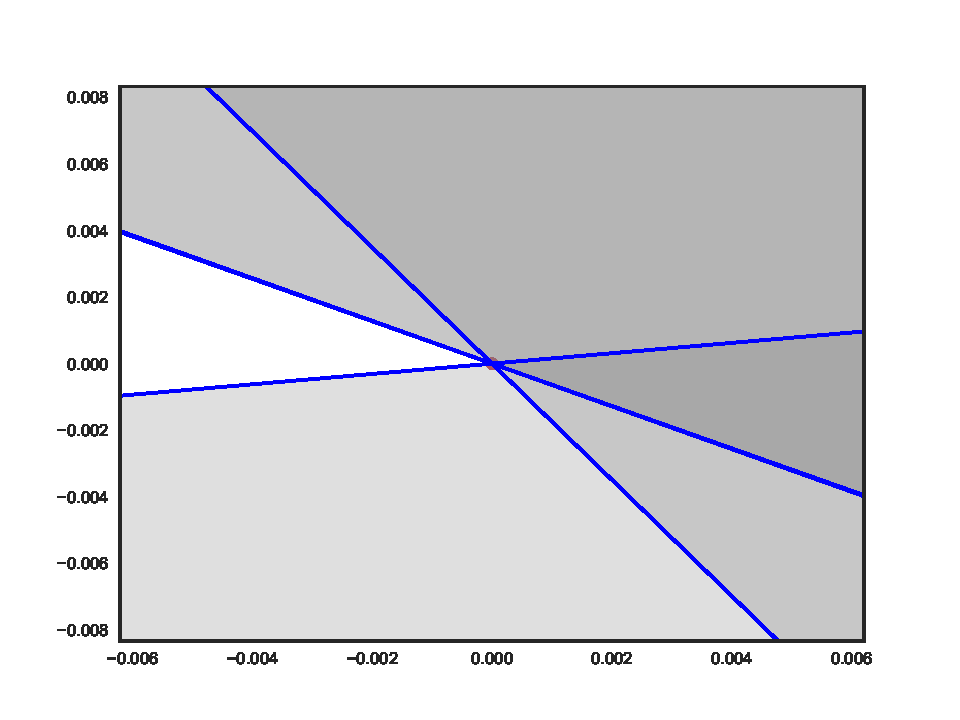
\includegraphics[width=\textwidth]{img/init/relu/conv2d_50-0.pdf}
        \caption{\ReLU 50th layer}
        \label{fig:reluInit501}
    \end{subfigure}
    ~ %add desired spacing between images, e. g. ~, \quad, \qquad, \hfill etc. 
    %(or a blank line to force the subfigure onto a new line)
    \begin{subfigure}[b]{0.3\textwidth}
        \includegraphics[width=\textwidth]{img/init/relu/conv2d_50-2.pdf}
        \caption{\ReLU 50th layer}
        \label{fig:reluIniti502}
    \end{subfigure}
    \\
    \begin{subfigure}[b]{0.3\textwidth}
        \includegraphics[width=\textwidth]{img/init/relu-bn/conv2d_1-0.pdf}
        \caption{\ReLUBN input layer}
        \label{fig:reluBNInitInput}
    \end{subfigure}
    ~ %add desired spacing between images, e. g. ~, \quad, \qquad, \hfill etc. 
      %(or a blank line to force the subfigure onto a new line)
    \begin{subfigure}[b]{0.3\textwidth}
        \includegraphics[width=\textwidth]{img/init/relu-bn/conv2d_50-0.pdf}
        \caption{\ReLUBN 50th layer}
        \label{fig:reluBNInit501}
    \end{subfigure}
    ~ %add desired spacing between images, e. g. ~, \quad, \qquad, \hfill etc. 
    %(or a blank line to force the subfigure onto a new line)
    \begin{subfigure}[b]{0.3\textwidth}
        \includegraphics[width=\textwidth]{img/init/relu-bn/conv2d_50-2.pdf}
        \caption{\ReLUBN 50th layer}
        \label{fig:reluBNInit502}
    \end{subfigure}
    \\
    \begin{subfigure}[b]{0.3\textwidth}
        \includegraphics[width=\textwidth]{img/init/layerwise/conv2d_1-0.pdf}
        \caption{\SepLayer input layer}
        \label{fig:layerwiseInitInput}
    \end{subfigure}
    ~ %add desired spacing between images, e. g. ~, \quad, \qquad, \hfill etc. 
      %(or a blank line to force the subfigure onto a new line)
    \begin{subfigure}[b]{0.3\textwidth}
        \includegraphics[width=\textwidth]{img/init/layerwise/conv2d_50-0.pdf}
        \caption{\SepLayer 50th layer}
        \label{fig:layerwiseInit501}
    \end{subfigure}
    ~ %add desired spacing between images, e. g. ~, \quad, \qquad, \hfill etc. 
    %(or a blank line to force the subfigure onto a new line)
    \begin{subfigure}[b]{0.3\textwidth}
        \includegraphics[width=\textwidth]{img/init/layerwise/conv2d_50-2.pdf}
        \caption{\SepLayer 50th layer}
        \label{fig:layerwiseInit502}
    \end{subfigure}
    \\
    \begin{subfigure}[b]{0.3\textwidth}
        \includegraphics[width=\textwidth]{img/init/unitpointwise/conv2d_1-0.pdf}
        \caption{\SepUnitPoint Input}
        \label{fig:unitpointInitInput}
    \end{subfigure}
    ~ %add desired spacing between images, e. g. ~, \quad, \qquad, \hfill etc. 
      %(or a blank line to force the subfigure onto a new line)
    \begin{subfigure}[b]{0.3\textwidth}
        \includegraphics[width=\textwidth]{img/init/unitpointwise/conv2d_50-0.pdf}
        \caption{\SepUnitPoint 50th layer}
        \label{fig:unitpointInit501}
    \end{subfigure}
    ~ %add desired spacing between images, e. g. ~, \quad, \qquad, \hfill etc. 
    %(or a blank line to force the subfigure onto a new line)
    \begin{subfigure}[b]{0.3\textwidth}
        \includegraphics[width=\textwidth]{img/init/unitpointwise/conv2d_50-2.pdf}
        \caption{\SepUnitPoint 50th layer}
        \label{fig:unitpointInit502}
    \end{subfigure}
    
  \caption{} 
  \label{fig:init} 
\end{figure*}





\begin{figure*}[h]
  \begin{center}
    \includegraphics[width=1.0\textwidth]{peaks}
      \caption{Evolution of training throughout epochs (cross-entropy, constraint loss, and accuracy). Left-hand axis show the accuracy metric (blue line) against the cross-entropy, and constraint loss in the right axis (orange line), for each epoch of the training phase in the horizontal axis.}
			\label{fig:peaks}
\end{center}
\end{figure*}





\subsubsection{Zero initialization}\label{subsec:zero}

We set the parameters to zero in an attempt to simplify initialization. We leave the responsibility of pulling the parameters from zero to the constraint, taking advantage of the fact of that the constraint gradient depend on the input of the units. However, we have two problems: (1) all the units in the layer will share the same gradient and will became the same and, (2) During the first iterations $\xi^+ = \xi^-$, so the gradient from the positive constraint will cancel with the negative.
In order to \emph{break symmetry} of the layers, we use Dropout \cite{dropout}. We find that Dropout has a very strong effect, harming convergence. This is why we choose to use Annealed Dropout \cite{dropoutAnnealing}, starting with a rate of 0.5 for 500 epochs with linear decay. We address the positive and negative constraints cancelling each other by introducing a variable to balance them, see \ref{eq:definitionOfRho}. 
See Figure \ref{fig:zeros} to see how the network evolves until finds a solution. We would like to remark that in this setup the training dynamics become particularly wild in a fashion similar to \ref{fig:peaks}, with several peaks in the constraint loss which ultimately lead to the readjustment of the planes so a solution can be found. Also, we find this process depends on the position of the hyperplanes set during the dropout annealing, introducing an stochastic behaviour that we would prefer to avoid. Finding another mechanism to \emph{break symmetry} would be interesing.



\begin{figure*}
  \centering
    \begin{subfigure}[b]{0.5\textwidth}
        \includegraphics[width=\textwidth]{img/zero/3000/09-conv2d_1-0.pdf}
        \caption{Input layer}
        \label{fig:zerosInput3000}
    \end{subfigure}
    ~ %add desired spacing between images, e. g. ~, \quad, \qquad, \hfill etc. 
      %(or a blank line to force the subfigure onto a new line)
    \begin{subfigure}[b]{0.5\textwidth}
        \includegraphics[width=\textwidth]{img/zero/3000/57-09-output.pdf}
        \caption{Output layer}
        \label{fig:zerosOutput3000}
    \end{subfigure}
    
      
  \caption{Zero initialization plus \SepUnitPoint and annealed dropout} 
  \label{fig:zeros} 
\end{figure*}


\subsection{Results concerning Accuracy}\label{subsec:accuracyResults}

To gauge accuracy between \ReLU, \ReLU +  batchnorm (\ReLUBN), and our proposal we tested all variants of our constraint using the same setup as \ref{subsec:classification}. We sampled $100$ points ($85$ for training and $15$). We used a 50x4 network. As hyper-parameters, we used learning rates $\gamma \in \{0.01, 0.001, 0.0001\}$, a batch size $bs = 85$, constraint loss parameter $\lambda = 0.01$ when needed, and set the number of epochs to $T = 2000$. We used the Glorot initialization scheme \cite{Glorot10Initialization}. 
 
We find how any of \SepConstraint versions show significant improvements over the \ReLU and \ReLUBN baselines (which yield \emph{trivial} validation accuracies of $40$\% and $60$\%, respectively). In the other hand, we see how \SepLayer achieves perfect accuracy closely followed by \SepUnitPoint, whereas \SepUnit and \SepPoint lag a bit behind, mirroring the results from \ref{subsec:classification}. The reader can observe Table \ref{tab:moons} for further detail.


\begin{table}[h!]
\begin{center}
\begin{tabular}{l|rr|rr}
\toprule
{}  & \multicolumn{2}{c}{Accuracy} & \multicolumn{2}{c}{Loss} \\
{}  & Train   & Val.  & Train  & Val.  \\
\midrule
\ReLU            &  0.5176 &      0.4 &  0.6925 &  0.6938 \\
\ReLUBN     &  0.8117 &      0.6 &  0.6331 &  0.6636 \\
\SepLayer &  1.0000 &      1.0 &  0.0000 &  0.0211 \\
\SepPoint    &  0.9294 &  0.8000 &  0.1765 &  0.6476 \\
\SepUnit    &  0.9058 &  0.8000 &  0.4161 &  1.5228 \\
\SepUnitPoint   &  0.9882 &  0.9333 &  0.6988 &  1.0810 \\
\bottomrule
\end{tabular}
\end{center}
\caption{Maximal performance experiment using the \moons dataset. From left to right, accuracy and loss (for \emph{train} and \emph{validation} sets) for \ReLU, \ReLUBN, and  \SepConstraint in all its variants.}
  \label{tab:moons}
\end{table}

